%%% General Relativity notes.

\documentclass{momento}
%\documentclass{article}
\usepackage{physicsplus}
%\usepackage{tensor}
%\usepackage{breqn}
%\usepackage{mathtools}
%\usepackage{microtype}

\title{General Relativity}
\author{Daniel Williams}


\usepackage{pgfplots}
\usepgfplotslibrary{polar}
\usetikzlibrary{calc}

%\usepackage{paracol}
%\usepackage{lipsum}
%\usetikzlibrary{calc}

%\usetikzlibrary{decorations.markings}
\providecommand{\Lag}{\mathcal{L}} %The Lagrangian
\providecommand{\Op}[1]{{\widehat{#1}}}  %A Quantum mechanical operator
\providecommand{\hcon}[1]{#1^{\dagger}}
\providecommand{\hOp}[1]{\hcon{\Op{#1}}}
\providecommand{\normbracket}[1]{\raisebox{0.1em}{:}  {#1}  \raisebox{.1em}{:}}
\providecommand{\nOp}[1]{\raisebox{0.1em}{:}  \Op{#1}  \raisebox{.1em}{:}}
\providecommand{\nhOp}[1]{\raisebox{0.1em}{:}  \Op{#1}  \raisebox{.1em}{:}}
\providecommand{\rn}{\mathbb{R}^n}
\providecommand{\of}[1]{\tilde{#1}}
\providecommand{\ld}[2]{\pounds_{\! #1}{#2}}
\providecommand{\ten}[1]{\mathsf{{#1}}}
\providecommand{\trt}[1]{{\mathop{#1}^{\text{\scriptsize{tt}}}}}

%\hypersetup{
%    colorlinks,
%    pdfborder={0 0 0},
%    linkcolor={muted-blue},
%    citecolor={blue!50!black},
%    urlcolor={blue!80!black}
%}

\begin{document}
\frontmatter

{
\thispagestyle{empty}
\begin{tikzpicture}[remember picture,overlay]
  \fill[fill=Maroon] (current page.south west) rectangle (current page.north east);
  %\fill[fill=white, yshift=-10cm]  (current page.north east) rectangle (current page.north west);
  \def\nbrcircles {377}
  \def\outerradius {30mm}
  \def\deviation {.9}
  \def\fudge {.62}

  \newcounter{cumulArea}
  \setcounter{cumulArea}{0}

  \pgfmathsetmacro {\goldenRatio} {(1+sqrt(5))}
  \pgfmathsetmacro {\meanArea} {pow(\outerradius * 10 / \nbrcircles, 2) * pi}
  \pgfmathsetmacro {\minArea} {\meanArea * (1 - \deviation)}
  \pgfmathsetmacro {\midArea} {\meanArea * (1 + \deviation) - \minArea}

  \foreach \b in {0,...,\nbrcircles}{
    % mod() must be used in order to calculate the right angle.
    % otherwise, when \b is greater than 28 the angle is greater
    % than 16384 and an error is raised ('Dimension too large').
    % -- thx Tonio for this one.
    \pgfmathsetmacro{\angle}{mod(\goldenRatio * \b, 2) * 180}

    \pgfmathsetmacro{\sratio}{\b / \nbrcircles}
    \pgfmathsetmacro{\smArea}{\minArea + \sratio * \midArea}
    \pgfmathsetmacro{\smRadius}{sqrt(\smArea / pi) / 2 * \fudge}
    \addtocounter{cumulArea}{\smArea};

    \pgfmathparse{sqrt(\value{cumulArea} / pi) / 2}
    \fill[opacity=0.3] (\angle:\pgfmathresult) circle [radius=\smRadius] ;
}  

  \node at (current page.center) [width=24cm, yshift=10cm] 
    {\color{white}\fontsize{72pt}{80pt}\center \selectfont\sffamily General Relativity};

  \node at (current page.south) [text width= \textwidth, yshift=5cm] 
    {\color{white}\fontsize{32pt}{120pt}\selectfont \sffamily Daniel Williams};

\end{tikzpicture}
}
\newpage

\maketitle
\makeglossary

\tableofcontents


\mainmatter
\part{Geometrical and Mathematical Methods}
\label{part:geometrical-methods}

\chapter{Basics}
\label{cha:basics}

\section{The topology of $\mathbb{R}^n$}
\label{sec:topology-mathbbrn}

The space $\rn$ is the usual $n$-dimensional space of vector algebra,
where a position can be described by a real $n$-tuple, $(x_1, x_2,
\dots, x_n)$. The local topology of $\rn$ is centred around the
concept of a neighbourhood of a point in $\rn$, and this allows the definition of a distance function between points, $\vec{x}$ and $\vec{y}$ in $\rn$,
\begin{equation}
  \label{eq:1}
  d(\vec{x},\vec{y}) = \qty[ (x_1 - y_1)^2 + (x_2 - y_2)^2 + \cdots + (x_n - y_n)^2 ]^{\half}
\end{equation}

\begin{definition}[Neighbourhood]
  A neighbourhood of a point $x$ in $X$ is a set $N(x)$ containing an
  open set which contains $x$.
\end{definition}
A family of neighbourhoods induces a notion of ``nearness'' to $x$.

A neighbourhood of radius $r$ of the point $\vec{x}$ in $\rn$ is thus
the set of points $N_r(\vec{x})$ with a distance less than $r$ from
$\vec{x}$. Such a neighbourhood is \emph{discrete} if each point has a
neighbourhood containing no other points; which is clearly untrue for
$\rn$, which is thus continuous.

A set of points $S$ in $\rn$ is \emph{open} if every point $x \in S$ has a
neighbourhood contained within $S$. The interval $a<x<b$ is an open
neighbourhood, but $a \leq x < b$ is closed, as the points $a=x$ have
neighbourhoods partially outside the set.

\begin{definition}[Hausdorff Space]
  A space is Hausdorff if any two distinct points in the space posess
  disjoint neighbourhoods.
\end{definition}

We can draw a line between two points in $\rn$, as we can have
neighbourhoods about each point which do not intersect, which is the
Hausdorff property of the space.

Using the distance function $d(\vec{x}, \vec{y})$ to define these
properties induces a topology on a space, enabling the definition of
open sets in the space, which have the properties
\begin{enumerate}
\item if $O_1$ and $O_2$ are open sets, then so is their intersection, $O_1 \cap O_2$
\item the union of any collection of open sets is open.
\end{enumerate}
To make (1) apply to all sets the empty set must be defined as open, and for (2) to work $\rn$ as a whole must be open.

\section{Mappings}
\label{sec:mappings}

A map from a space $M$ to a space $N$ is a rule which associates
elements $x \in M$ to elements $y \in N$. The simplest map is a
function $f:\mathbb{R} \to \mathbb{R}$ taking $x \mapsto f(x)$. 

Some terminology for mappings of the form $f:M \to N$,
\begin{description}
\item[image] the set, $T$ of elements from the set $N$ which are mapped to from elements of $S \subset M$. Denoted $f(S)$.
\item[inverse-image] the set $S$
\end{description}
There are a number of types of mapping.
\begin{description}
\item[Many-to-one] a map where multiple elements of $S$ map to the same element of $T$ 
\item[one-to-one] a map where only one element of $S$ maps to each element of $T$
\item[inverse] a map which takes $T \to S$, and is only well-defined for one-to-one maps
\end{description}

Let $f:M \to N$ and $g: N \to P$, then the operation of function composition is defined as 
\[ g \circ f : M \to P \]

A map $f:M \to N$ is continuous at $x \in M$ if any open set of $N$
containing $f(x)$ contains the image of an open set of $M$, provided
$M$,$N$ are topological spaces. $f$ is continuous on $M$ if it is continuous at all the points in $M$.

If $f(x_1, \dots, x_n)$ is a function which is defined on an open
region $S$ of $\rn$ the it is \emph{differentiable of class} $C^k$ if
all its partial derivatives of the order less or equal to $k$ exist
and are themselves continuous on $S$; $f$ is a $C^k$ function.

\section{Real Analysis}
\label{sec:real-analysis}

A real function is analytic if, at $x=x_0$ it has a Taylor expansion
about $x_0$ which converges to $f(x)$ in a neighbourhood of $x_0$,
{\small
\begin{align}
  \label{eq:2}
  f(x) &= f(x_0) + (x-x_0) \eval{\dv{f}{x}}_{x_0} 
        + \half (x-x_0)^2 \eval{\dv[2]{f}{x}}_{x_0}
       %&\quad + \frac{1}{3!} (x-x_0)^3 \eval{\dv[3]{f}{x}}_{x_0} 
       + \cdots
\end{align}
} This clearly requires that $f$ be infinitely differentiable, but
this is not a guarantee that $f$ is analytic, e.g. $\exp(-1/x^2)$
which is non-analytic as a real function, but becomes analytic with a
singularity at $z=0$ as a complex function.

A real-valued function $g(\cdots)$ defined on an open region $S$ of $\rn$ is square-integrable if 
\begin{equation}
  \label{eq:3}
  \int_S \qty[ g(x_1, \dots, x_n)]^2 \dd{x_1 \dots \dd{x_n}}
\end{equation}
exists. A square-integrable function can be approximated by an analytic function $g'$ such that the integral of $(g - g')^2$ over $S$ can be made arbitrarily small.

A $C^{\infty}$ function need not be analytic, so an analytic function
is denoted $C^{\omega}$.

An operator $A$ acts on functions defined on $\rn$, and takes one function, $f$, into another one, $A(f)$. Examples are multiplication, differentiation, and fixed-kernel integration.
The commutator of two operators is defined
\begin{equation}
  \label{eq:4}
  [A,B](f) = (AB-BA)(f)
\end{equation}

%%% Local Variables: 
%%% mode: latex
%%% TeX-master: "../project"
%%% End: 


\chapter{Manifolds and Tensors}
\label{cha:manifolds-tensors}


\section{Manifolds}
\label{sec:manifolds}

$\rn$ is the set of all $n$-tuples of real numbers. A set $M$ is
defined to be a manifold if each element of $M$ has an open
neighbourhood with a continuous bijection onto an open set of $\rn$
for some $n$. This mathematical object is rather degenerate, and
hasn't got, for example, a notion of distance, and what structure is
defined is only at a local level.

The elements, $P$ of $M$ have a unique $n$-tuple, the co-ordinates of
$P$:
\begin{equation}
  \label{eq:5}
  \qty( x_1(P), x_2(P), \dots, x_n(P) )
\end{equation}

\begin{figure}[b]
  \centering
  \begin{tikzpicture}[scale=0.45]
\begin{scope}[xshift=-50]
	\shade[left color=muted-blue!10,right color=muted-blue!80] 
	  (0,0) to[out=-10,in=150] (6,-2) -- (12,1) to[out=150,in=-10] (5.5,3.7) -- cycle;

	\begin{scope}[scale=0.4, xshift=300]
		\coordinate (A) at (0,0);
		\draw node at (6, -0.5) {$U$};
		\fill[opacity=0.1, fill=black, dotted] 
		  (0,0) to[out=-10,in=150] (6,-2) -- (12,1) to[out=150,in=-10] (5.5,3.7) -- cycle;
	\end{scope}
	\begin{scope}[scale=0.3, xshift=400, yshift=100]
		\coordinate (B) at (12,1);
		\draw node at (6, 2.5) {$V$};
		\fill[opacity=0.1, fill=black, dotted] 
		  (0,0) to[out=-10,in=150] (6,-2) -- (12,1) to[out=150,in=-10] (5.5,3.7) -- cycle;
	\end{scope}
\end{scope}

\begin{scope}[yshift=-250, xshift=-50]
	\coordinate (C) at (0, 2.5);
	\draw [->] (0,0) -- (5,0); \draw [->] (0,0) -- (0,5); \fill [opacity=0.1] (0,0) rectangle (5,5);
	\fill [opacity=0.1] (3,3) rectangle (5,5);
	\draw (2.5,.5) node {$f_U(u)$};
\end{scope}
\begin{scope}[yshift=-250, xshift=200]
	\coordinate (D) at (5,2.5);
	\coordinate (E) at (1,1);
	\draw [->] (0,0) -- (5,0); \draw [->] (0,0) -- (0,5); \fill [opacity=0.1] (0,0) rectangle (5,5);
	\fill [opacity=0.1] (0,0) rectangle (2,2);
	\draw (2.5,4.5) node {$f_V(v)$};
\end{scope}

\draw [ultra thick, accent-red]  (A) edge [out=180, in=180, ->] node [black, fill=white, pos=0.3]  {$f_U$} (C) ;
\draw [ultra thick, accent-blue]  (B) edge [out=0, in=0, ->] node [black, fill=white, pos=0.4]  {$f_V$} (D);

\draw [ultra thick, accent-green] (C)+(4,1.5) edge [out=0, in=180,->] node [black, fill=white, pos=0.5]  {$f_V \circ f^{-1}_U$} (E);
\end{tikzpicture}
%%% Local Variables: 
%%% mode: latex
%%% TeX-master: "../project"
%%% End: 

  \caption{Open sets $U$ and $V$ of a manifold which can be mapped, by the functions $f_U$ and $f_V$ onto open sets in $\mathbb{R}^n$, $f_U(u)$ and $f_V(v)$.}
  \label{fig:manifolds}
\end{figure}

Let $f:U(P) \to \rn$ be a function from a neighbourhood $U$ around
$P\in M$ of $M$ onto an open set $f(U) \in \rn$, then the pair,
$(U,f)$ are a chart. The open neighbourhoods must overlap if all
points of $M$ must be included in at least one, and so these overlaps
give an additional characterisation of the manifold. Suppose $V$ is a
neighbourhood overlapping $U$, such that $V$ has a map $g$ onto an
open region of $\rn$, this region may be completely disjoint from the
equivalent region for $U$. The open intersection of $U$ and $V$ is
described by two coordinate systems, so there should be an expression
connecting the two. Such an equation is a \emph{coordinate
  transformation}.

\begin{definition}[Manifold]
  A manifold is a second-countable Hausdorff space which is locally
  homeomorphic to Euclidean space.
\end{definition}
\begin{definition}[Chart]
  A chart $(U, f_U)$ of a manifold is an open set $U$ together with a
  mapping $f_U: U \to \rn$.
\end{definition}
\begin{definition}[Coordinates]
  The coordinates $(x^1, \cdots, x^n)$ of the image $f_U(x) \in \rn$
  are the coordinates of $x$ in the chart $(U, f_U)$; the local
  coordinate system.
\end{definition}

If a whole system of charts, an atlas, can be constructed such that
every point in $M$ is in at least one neighbourhood, and every chart
is $C^k$-related to every overlapping neighbour the manifold is
$C^k$. Any such manifold for $C^1$ or greater is a differentiable
manifold.

Many mathematical spaces can be considered as manifolds, for example
the space of Lorentz boosts, mechanical phase space, solution spaces
for functions, and vector spaces. Groups also have representations as
manifolds; a Lie group, e.g. the group of rotations of a rigid object
in space is also a $C^{\infty}$ manifold.

\begin{figure}[b]
  \centering
  
\newcommand{\mobstrip}[1]{%
\draw [very thick, top color=white,
       bottom color=muted-blue, rotate=#1,
       draw=muted-blue
      ]
 (0:2.8453)    ++ (-30:1.5359) arc (60:0:2)
            -- ++  (90:5) arc (0:60:2) 
            -- ++ (150:3) arc (60:120:2) 
            -- ++ (210:5) arc (120:60:2) -- cycle;
}%

\begin{tikzpicture} [rotate=22, scale=0.5]
   \begin{scope} [transform shape]
     \mobstrip{0}
     \mobstrip{120}
     \mobstrip{-120}
     \draw [
     ultra thick, accent-red,
     decoration={markings, mark=at position 0.625 with {\arrow{>}}},
        postaction={decorate}
     ] (-60:3.5) circle (1);
     \draw [
     ultra thick, accent-red,
          decoration={markings, mark=at position 0.625 with {\arrow{<}}},
        postaction={decorate}
     ](180:3.5) circle (1);
  %   % redraw the first strip after clipping
  %   \clip (-1.4,2.4)--(-.3,6.1)--(1.3,6.1)--(5.3,3.7)--(5.3,-2.7)--cycle;
  %   \strip{0}
  %   \draw (60:3.5) node [gray,xscale=-4,yscale=4,rotate=30]{b};
   \end{scope}
\end{tikzpicture}
%%% Local Variables: 
%%% mode: latex
%%% TeX-master: "../project"
%%% End: 

  \caption{The M\"obius strip, a non-orientable manifold; as such,
    there is no consistent notion of a clockwise or an anti-clockwise
    orientation across the whole manifold.}
  \label{fig:mobius}
\end{figure}

\begin{definition}[Orientability]
  Let $M^n$ be a differentiable $n$-dimensional manifold equipped with
  an atlas $\set{\phi_a}$, and suppose that for any two charts of the
  atlas, $\phi_{\alpha}$, and $\phi_{\beta}$ the Jacobian of the
  transition function $\phi_{\beta \alpha} = \phi_{\beta} \circ
  \phi_{\alpha}^{-1}$ is positive at all points in the domain, then
  $M$ is an orientable manifold.
\end{definition}
A Jacobian which is negative will reverse the orientation of a
coordinate system.

\section{Global Properties}
\label{sec:global-properties}

At a local level all manifolds look like $\rn$, but on a global level
this is not the case. For example a sphere, $S^2$ and a crayon are
both two-dimensional manifolds, and neither has a single map to
$\mathbb{R}^2$, but there is a continuous map from one to the other.
If there is a $C^{\infty}$ bijective map from one $C^{\infty}$
manifold to another, then the two map is a \emph{diffeomorphism} from
one manifold to the other.

\begin{figure}[t]
  \centering
  \begin{tikzpicture}[scale=0.45]
    \begin{scope}[yshift=120]
      \draw[ultra thick, muted-green] (0,0) -- (10,0); 
      \node at (-1.2,0) {$\lambda \in \mathbb{R}^1$} ;
      \foreach \coor in {0,1,...,10}
      \coordinate (re\coor) at (\coor, 0);
    \end{scope}
    \begin{scope}[xshift=-50]
	\shade[left color=muted-blue!10,right color=muted-blue!80] 
	  (0,0) to[out=-10,in=150] (6,-2) -- (12,1) to[out=150,in=-10] (5.5,3.7) -- cycle;

	\begin{scope}[scale=0.4, xshift=300]
		\coordinate (A) at (0,0);
		\draw node at (11.5, 0.8) {$U$};
		\fill[opacity=0.1, fill=black, dotted] 
		  (0,0) to[out=-10,in=150] (6,-2) -- (12,1) to[out=150,in=-10] (5.5,3.7) -- cycle;
	\end{scope}

\draw[muted-orange,line width=1.5pt,shorten >= 3pt,shorten <= 3pt] 
  (0,0) .. controls (6,-0.2) and (5,1.5) ..
  coordinate[pos=0.0] (cux0)
  coordinate[pos=0.1] (cux1) 
  coordinate[pos=0.2] (cux2) 
  coordinate[pos=0.3] (cux3) 
  coordinate[pos=0.4] (cux4) 
  coordinate[pos=0.5] (cux5) 
  coordinate[pos=0.6] (cux6) 
  coordinate[pos=0.7] (cux7) 
  coordinate[pos=0.8] (cux8) 
  coordinate[pos=0.9] (cux9) 
  coordinate[pos=1.0] (cux10) (12,1);
\draw (cux10)+(0.3,0) node [right] {$P \in M$};

% we draw the filled red circles on the red line
\foreach \coor in {0,1,...,10}{
  \draw (cux\coor) edge  [accent-blue, shorten >=0.1cm, 
                          shorten <= 0.1cm, line width=0.3mm, 
                          <-, out=90, in=270] 
        (re\coor);
  \draw[fill=muted-green, draw=white] (re\coor) circle (3pt);
  \draw[fill=muted-orange, draw=white] (cux\coor) circle (3pt);
}
\draw (13, 3) node {$f$};
\draw (3, -2) node {$g$};
\end{scope}
\begin{scope}[yshift=-210, xshift=-50]
	\coordinate (C) at (0, 0.5);
	\draw [->] (0,0) -- (12.1,0); 
        \draw [->] (0,0) -- (0,5); 
        \fill [opacity=0.1] (0,0) rectangle (12,5);
        \draw (10,0.5) node {$g(U) \in \mathbb{R}^n$};
        \node (E) at (12, 4);

        \draw [ultra thick, accent-green, out=0, in=180] 
        (0, 0.5) edge % [out=0, in=180] 
          coordinate[pos=1/10] (cdx4)
          coordinate[pos=3/10] (cdx5)
          coordinate[pos=6/10] (cdx6)
          coordinate[pos=9/10] (cdx7)
        (8, 5);
\end{scope}

\foreach \coor in {4,5,...,7}{
 %\draw[fill=muted-green, draw=white] (re\coor) circle (3pt);
  \draw[fill=accent-green, draw=white] (cdx\coor) circle (3pt);
}

\foreach \coor in {4,5,...,7}{
   \draw (cux\coor) edge  [accent-red, shorten >=0.1cm, 
                           shorten <= 0.1cm, line width=0.3mm, 
                           ->, out=270, in=90] 
         (cdx\coor);
}


\end{tikzpicture}
\caption{A curve defined over a manifold.}
  \label{fig:manifold-curve}
\end{figure}

\section{Curves and Functions on Manifolds}
\label{sec:curves}

A curve is a differentiable mapping from an open set of $\mathbb{R}^1$
into $M$, so each point $\lambda$ on the real line is associated with
a point in $M$.

A function on $M$ is a rule assigning a real number to each point of
$M$. When a region of $M$ is mapped to $\rn$ the function becomes a
function of $\rn$. If this is differentiable on $\rn$ it is defined as
being differentiable on $M$. That is
\[ g(P \in M) = g(x_1(P), \dots, x_n(P)) = g(x_1, \dots x_n) \]

Now, consider a curve, $c$, which passes through $P \in M$, which is
described by $x^i = x^i(\lambda)$ for $i \in \set{1, \dots, n}$, and a
differentiable function $g(x^i)$ on $M$. $g$ has a value at each point
along the curve, so there is a differentiable function, $g(\lambda)$
along the curve which gives the value of $c$ at the point with a parameter value $\lambda$,
\[ g(\lambda) = g(x^1(\lambda), \dots, x^n(\lambda) ) =
g(x^i(\lambda)) \]
Differentiating, and applying the chain rule,
\begin{equation}
  \label{eq:6}
  \dv{g}{\lambda} = \dv{x^i}{\lambda} \dv{g}{x^i}
\end{equation}
using Einstein notation.

In Euclidean space the set $\set{ \dv*{x^i}{\lambda} }$ would be
components of a vector tangent to the curve $x_i(\lambda)$, and would
be the tangent to an infinite number of curves through $P$.

Manifolds do not necessarily have a notion of distance between points,
so vectors must be defined in terms only of infinitessimal
neighbourhoods of the points of $M$. 

\section{Vectors}
\label{sec:vectors}

Suppose $a$ and $b$ are two numbers and $x^i = x^i(\mu)$ is another curve through $P$, then at $P$,
\[ \dv{\mu} = \dv{x^i}{\mu} \pdv{x^i} \]
and
\[ a \dv{\lambda} + b\dv{\mu} = \qty( a \dv{x^i}{\lambda} + b \dv{x^i}{\mu} ) \pdv{x^i} \]
The numbers inside the bracket are the components of a new vector, tangent to a curve at $P$, so a curve must exist, with parameter $\phi$ such that at $P$,
\[ \dv{\phi} = \qty( a \dv{x^i}{\lambda} + b \dv{x^i}{\mu} ) \pdv{x^i} \]
collecting this, at $P$,
\[ a \dv{\lambda} + b \dv{\mu} = \dv{\phi} \]
forming a vector space.

In any given coordinate system there are special curves, the
coordinate lines. The derivations along them are $\pdv*{x^i}$, and
$\dv*{\lambda}$ has components on the basis, showing that
$\set{\dv*{x^i}{\lambda}}$ are a basis for a vector space.

\section{Basis Vectors and basis vector fields}
\label{sec:basis-vectors-basis}

At any point $P$ the space $T_P$ is a vector space with the same
dimension $n$ as the manifold, and is the tangent space. Any
collection of linearly independent vectors can form a basis, and if
there is a coordinate system $\set{x^i}$ in a neighbourhood $U$ of $P$
then these coordinate define a coordinate basis at all points in $U$.

\begin{definition}[Tangent Vector]
  Let $M^m$ be a differential manifold, $p$ a point on it, and $U$ be
  an open neighbourhood of $M$. Let $\epsilon>0$, and $\gamma :
  (-\epsilon, \epsilon) \to U$ be a differentiable curve on $M$ such
  that $\gamma(0) = p$. For any differentiable function $f:U \subset M
  \to \mathbb{R}$ the directional derivative of $f$ along $\gamma$ to
  be the number
  \[ D_{\gamma}(f) = \eval{\dv{t}( f (\gamma(t) ) )}_{t=0} \] The
  operator $D_{\gamma}$ is called the tangent vectorto $\gamma$ at
  $p$.
\end{definition}
\begin{definition}[Tangent Space]
  The tangent space of $M$ at $p$, $T_p$ is a vector space with the
  same dimension as the manifold composed of all of the tangent
  vectors to the manifold at $p$. If $x$ is a coordinate system which
  contains $p$, then the set of $\pdv*{x}$ are the basis of the tangent
  space; and this is a coordinate basis.
\end{definition}

At any point $P$ an arbitrary vector $\vec{V}$ is
\[ \vec{V} = V^i \pdv{x^i} = V^j \bar{e}_j = V^j \partial_j\] for an
arbitrary basis $\set{\vec{e}_i}$. Thus $\set{V^i}$ are the components
of $\vec{V}$ in $\set{ \pdv*{x^i}}$, and $\set{V^j}$ the components in
$\vec{e}_j$, where a useful notation, $\partial_i \equiv \pdv*{x^i}$ is
introduced.

\section{Differential of a map}
\label{sec:differential-map}

\begin{definition}[Differential]
  Let $\phi: M^m \to N^n$ be a differentiable map between
  differentiable manifolds. We define the differential of $\phi$ at $p
  \in M$ as the linear transformation between vector spaces
  \begin{align*}
    \dt{\phi_p} : T_pM & \to T_{\phi(p)N} \\
D_{\gamma} &\mapsto D_{\phi \circ \gamma}
  \end{align*}
\end{definition}

\section{Fibre bundles}
\label{sec:fiber-bundles}



\begin{figure}[b]
  \centering
  \begin{tikzpicture}
  \draw [thick, ->] (1,0) -- (7.5,0);
  \node at (8,0) {$B$};

  \draw [thick, ->] (0,0.5) -- (0,3);
  \node at (0.5, 3) {$\mathbb{R}^n$};

  \fill [opacity=0.1] (1,0.5) rectangle (7, 3);
  \node at (6.5,2.7) {$E$};
  \foreach \x in {3,3.5,...,6}{
    \draw (\x, 0.5) -- (\x, 3);
  }

  \draw (7, 1.5) edge [shorten >=0.1cm, shorten <=0.1cm, ->, 
                       accent-red, out=0, in=90, thick]
   node [midway, right] {$\pi$} (7.3,0);

   \draw [<->] (3,-0.25) -- (6,-0.25) node [midway, fill=white] {$U$};
   \draw (3,0) node {$($}; \draw (6,0) node {$)$};
   \filldraw [fill=white] (4.5,0) circle (0.07) node [above] {$x$};
   \draw (4.5, 3.5) node {fibre $\pi^{-1}(x)$} edge [thick, accent-blue, ->] (4.5, 3);
\end{tikzpicture}


%%% Local Variables: 
%%% mode: latex
%%% TeX-master: "../project"
%%% End: 

  \caption{A fibre bundle, $E$, over a base $B$, with a projection
    function $\pi$. Each fibre at a point $x \in B$ is then described
    by a function $\pi^{-1}(x)$, and the whole bundle over an open
    region $U$ is  $\pi^{-1}(U)$.}
  \label{fig:fibre-bundle}
\end{figure}

\begin{definition}[Homeomorphism]
A homeomorphism is an bijection from one space to the other which is
continuous, and its inverse is continuous.
\end{definition}

\begin{definition}[Fibre Bundle]
A fibre bundle is a space, $E$, which has a base manifold $B$, a
projection $\pi: E \to B$, a typical fibre $F$ a structure group $G$
of homeomorphisms of $F$ onto iteself, and a family $\set{U_j}$ of
open sets which cover $B$, which satisfy
\begin{enumerate}
\item Locally the bundle is trivial: the bundle over any set $U_j$
  which is just $\pi^{-1}(U_j)$ has a homeomorphism onto $U_j \times
  F$. Part of this is a homeomorphism from each fibre, say
  $\pi^{-1}(x)$, $x\in B$ onto $F$. Call this map $h_j(x)$ labelled
  both by $x$ defining the fibre, but also by $j$ indexing the set
  $U_j$ which contains $x$.
\item When two sets $U_j$ and $U_k$ overlap a point $x$ in their
  intersection has two homeomorphisms, $h_j(x)$ and $h_k(x)$ from the
  fibre onto $F$. Thus $h_j(x) \circ h_k^{-1}(x)$ is a homeomorphism
  of $F$ onto $F$. This must be an element of $G$.
\end{enumerate}
\end{definition}

In two overlapping neighbourhoods there are homeomorphisms $h_j(x)$
and $h_k(x)$ which map $\vec{v}$ to $\alpha_{(j)}$ and to
$\alpha_{(k)}$, and so the homeomorphism $h_j(x) \circ h_k^{-1}(x): F
\to F$ maps $\alpha_{(k)} \to \alpha_{(j)}$, which is equivalent to
multiplication by a real number $r_{jk} = \alpha_{(j)}/a_{(k)}$, which
must be a non-zero real number. Thus the structure group is
$\mathbb{R}^1 - \set{0}$, which is a Lie group under multiplication.

The difference between two bundles over a base space is the bundles'
\emph{structure group}.

If the coordinates $\lambda_j$ can be arranged in such a way that
$\lambda_j$ and $\lambda_k$ increase in the same direction in $S^1$ in
the overlap region, then $S^1$ is orientable. In such an overlap all
$r_{jk}$ are positive, so the structure group becomes $\mathbb{R}^+$,
and by scaling the coordinates so that $\dv*{\lambda_j}{\lambda_k} =
1$ in every overlap the group reduces to the identity element, thus
the structure group is trivial and we have a bundle structure.

Consider the combination of a manifold $M$ with all of its tangent
spaces $T_P$. This is equivalent to the set of all vectors at all
points in the manifold, and can be defined as a new manifold $TM$; a
\emph{fibre bundle}, with the fibres the spaces $T_P$, and has
dimension $m+n$, with $m$ the dimension of each fibre, and $n$ of the
base manifold. An example of a fibre bundle is the structure of space
and time in the Newtonian world view, where the base space is
$\mathbb{R}^1$, with $\mathbb{R}^3$ fibres, that is a base of time
with fibres of space. This follows, as there is no absolute concept of
space in Newtonian physics, and so there is no connection between
points on each fibre.

\begin{definition}[Cartesian Product Space]
A Cartesian product space of two spaces $M$ and $N$, denoted $M \times
N$ is the set of all ordered pairs $(a,b)$ for $a \in M$ and $b \in
N$, and if $M$ and $N$ are manifolds then $M \times N$ is also a
manifold; the set of coordinates $\set{x^i}$ of an open set $U$ of $M$
taken with $\set{y^i}$ of an open set $V$ of $N$ form a set of $m+n$
coordiates for the open set $(U,V)$ of $M \times N$.
\end{definition}

Fiber bundles are locally product spaces; they are locally trivial, as
they look like product spaces, but not usually globally trivial. For
example, $TS^2$ is the tangent bundle of a 2-sphere; were it globally
tivial there would be a diffeomorphism of $TS^2$ onto $S^2 \times
\mathbb{R}^2$. Consider the set $(P, \bar{V})$ in the product space;
the invserse map gives a nowhere-zero cross-section of $TS^2$, but a
vector field must always have a zero, and so $TS^2$ has no global
product structure. A tangent bundle $TS^1$ \emph{is} identical to $S^1
\times \mathbb{R}$, but if the circle is cut at a point $P$, and a
twist is introduced, making a M\"obius strip, the resulting bundle is
not a product space, as no bijection exists from one bundle onto all
of the other.

\begin{definition}[Tangent Bundle]
  Let $M^n$ be a differentiable manifold. The disjoint union of all
  tangent planes to $M$, \[ \coprod_{p \in M} T_p M \] is a vector
  bundle with the fibre $\rn$ over $M$, called the tangent bundle to
  $M$, denoted $TM$.
\end{definition}

\section{Integral Curves}
\label{sec:vector-fields}

For a $C^1$ vector field there is always a curve which has the field as a tangent at each of its points; these are its integral curves.

Let the components of the field be $V^i(P) = v^i(x^j)$ in a coordinate
system $\set{x^i}$ The statement that this is a tangent vector to a curve parameterised by $\lambda$ is
\begin{equation}
  \label{eq:7}
  \dv{x^i}{\lambda} = v^i(x^j)
\end{equation}
which is a set of first-order ODEs for $x^i(\lambda)$, which always
has a unique solution in a neighbourood of $P$.

\section{Lie Brackets}
\label{sec:lie-brackets}

Any linearly independent set of vector fields can serve as a basis,
but not all come from coordinate systems; all coordinate systems commute, but in general not all vector fields commute, and the commutator,
\[ \comm{V}{W} = V W - W V \] is a vector field with, in general,
non-vanishing components. If $W$ and $V$ are elements of a basis they
cannot be expressed as derivatives with respect to any
coordinates. The commutator is the Lie Bracket of the two vector
fields, and shows that the parameterisation of the integral curves of
these vector fields is not that of a coordinate system.

\begin{definition}[Lie Bracket]
  Let $X$ and $Y$ be vector fields of class $C^1$, then the Lie
  Bracket is a vector field, defined by the operation $f \mapsto (XY -
  YX) f$, and is denoted $\comm{X}{Y}$.
\end{definition}

The vector $\comm{V}{W}$ can be viusualised as the difference in
moving a distance $\Delta \lambda = \epsilon$ along the $V$ curve,
then $\Delta \mu = \epsilon$ along a $W$ curve, ending at a point
$A$. Going in the opposite order we end at a point $B$. The vector
between these two points is $\epsilon^2 \comm{V}{W}$.

A Lie Algebra of vector fields on a region $U$ of $M$ is a set $A$ of
vector fields on $U$ which is a vector space under addition, which is
closed under the Lie Bracket operation.

For a basis to be a coordinate basis the fields of the basis must commute,
\[\comm{A}{B} = 0 \]

\begin{figure}[t]
  \centering
  \begin{tikzpicture}[scale=0.7]

\begin{scope}[]
	\draw [thin, ->] (-.2, 0) -- (5.2,0);
	\draw [thin, ->] (0, -.2) -- (0,5.2); 

\clip (0,0) rectangle (5,5);
\draw [help lines] (0,0) grid (5,5);

	\draw [accent-red, ultra thick, ->] (1,1) -- (4,1) node [left, midway, below, black] {$\partial_\mu$};
	\draw [accent-red, ultra thick, ->] (1,4) -- (4,4) node [left, midway, above, black] {$\partial_\mu$};

	\draw [accent-blue, ultra thick, ->] (1,1) -- (1,4) node [left, midway, black] {$\partial_\nu$};
	\draw [accent-blue, ultra thick, ->] (4,1) -- (4,4) node [right, midway, black] {$\partial_\nu$};
\end{scope}

\begin{scope}[xshift=170]
 {

	}
	\draw [thin, ->] (-.2, 0) -- (5,0);
	\draw [thin, ->] (0, -.2) -- (0,5); 

	\draw [accent-red, ultra thick, ->] (1,1) -- (4,2) node [left, midway, below, black] {$W$};
	\draw [accent-red, ultra thick, ->] (1,4) -- (4,5) node [left, midway, above, black] {$W$};

	\draw [accent-blue, ultra thick, ->] (1,1) -- (1,4) node [left, midway, black] {$V$};
	\draw [accent-blue, ultra thick, ->] (4,2) -- (5,5) node [right, midway, black] {$V$};

\clip (0,0) rectangle (5,5);
	\clip (-.2,-.2) rectangle (5.5,5.2);
		\foreach \x in {0,0.55,...,4}{
		\draw [help lines] (\x-.06, 0) -- (\x+\x-1.2,6);
	}
	\foreach \y in {0.3,...,6}{
		\draw [help lines] (0,\y-0.6) -- (6, \y+1.3);
	}	



\end{scope}

\end{tikzpicture}
  \caption{A geometrical interpretation of the commutator. In the top diagram are two commuting vector fields, but in the lower diagram the two fields do not commute. Moving a distance $\epsilon$ along $V$ then $\epsilon$ along $W$ does not take us to the same place as moving $\epsilon$ along $W$ and then $\epsilon$ along $V$, so the paths do not meet, with a gap equal to $\epsilon^2\comm{V}{W}$ separating their end points.}
  \label{fig:commutator}
\end{figure}

\section{One-forms}
\label{sec:one-forms}

Consider $T_P$, the tangent space of vectors at a point $P$. A
one-form, $\of{\omega}$ at $P$ associates a vector $\vec{V}$ at P to a
real number, $\of{\omega}(\vec{V})$. 

\begin{subequations}
This function is linear; for vectors $\vec{V}$ and $\vec{W}$, and real numbers $a$ and $b$,
\begin{equation}
\label{eq:8}
 \of{\omega}( a \vec{V} + b \vec{W} ) = a \of{\omega}(\vec{V}) + b
\of{\omega}(\vec{W}) 
\end{equation}
can be multiplied by scalars,
\begin{equation}
  \label{eq:9}
  (a \of{\omega})(\vec{V}) = a [ \of{\omega}(\vec{V})]
\end{equation}
and have the property
\begin{equation}
  \label{eq:10}
  (\of{\omega} + \of{\sigma}) (\vec{V}) + \of{\omega}(\vec{V}) + \of{\sigma}(\vec{V})
\end{equation}
\end{subequations}
They satisfy the axioms of a vector space, and are indeed the duals of vectors, and have a tangent vector space $T^{*}_P$.

A field of one-forms can represent the gradient of a function $f$;
such a field is denoted $\dd{f}$,
\[ \of{\dd{}}f (\dv*{\lambda}) = \dv{f}{\lambda} \]

In the vector space $T^{*}_P$ any $n$ linearly independent one-forms
can constitute a basis, however selecting a set of basis vectors,
$\set{\vec{e}_i}$ in $T_P$ induces a preferred basis on $T^{*}_P$, the
dual basis $\set{\of{\omega}^i}$.

These have the property
\[ \of{\omega}^i(\vec{e}_j) = \delta^i_j \]

\section{Tensors}
\label{sec:tensors}

\newcommand{\tensororder}[2]{#1 \choose #2}

Consider a point $P$ in a manifold $M$, a \emph{tensor} of type
$\tensororder{N}{N'}$ at $P$ is a linear function with $N$ one-form
arguments, and $N'$ vector arguments, which has a real scalar
value. Tensors are linear on every argument.

A $\tensororder{N}{N'}$ tensor field is a rule which assigns a
$\tensororder{N}{N'}$ tensor to each point in a space, and are
functions on $M$.

It is possible to construct higher-order tensors out of lower order
ones with the tensor (outer) product operation; for two vectors $V$
and $W$ the tensor product is defined such that
\begin{equation}
  \label{eq:11}
  V \otimes W (\of{p}, \of{q}) := V(\of{p}) W(\of{q})
\end{equation}

If the basis vectors and one-forms are given as arguments to the
tensor the components of the tensor are returned.

It is also possible to reduce the dimensionality of a tensor by a
process called \emph{contraction} whereby an entire argument is
removed from the tensor by constructing an inner product of those
parts of the tensor with either a one form or a vector.

\section{Basis Transformations}
\label{sec:basis-transf}

Consider a point $P$ in a manifold $M$, where a vector basis
$\set{e_i}$ is defined, but we want to switch to a description in
another basis, $\set{e_{j'}}$, then in $T_P$ there is a linear
transformation, $\Lambda$ between the old and the new basis,
\begin{equation}
  \label{eq:12}
  e_{j'} = \Lambda^i_{j'} e_i 
\end{equation}
where $\Lambda$ is non-singular, but arbitrary. It is not a tensor,
since its indices refer to different bases. The transformation matrix has an inverse, $\Lambda^{k'}_j$ such that
\[ \Lambda^{k'}_j \Lambda^j_i = \delta^{k'}_{i'} \] We require the
inverse transformation for basis one-forms, as is evident from the
relation
\[ \of{\omega}^i e_{j'} = \delta^{i}_{k} \Lambda^k_{j'} =
\Lambda^i_{j'} \]

The general expression for the change of coordinates of a tensor takes
the form
\begin{equation}
  \label{eq:71}
  \tensor{A'}{^{u_1\dots u_l}_{r_1 \dots r_m}} = \Lambda_{t_1}^{u_1} \cdots \Lambda_{t_l}^{u_l} \Lambda_{r_1}^{q_1} \cdots \Lambda_{r_m}^{q_m} \tensor{A}{^{t_1 \dots t_l}_{q_1 \dots q_m}}
\end{equation}

\section{The Metric Tensor}
\label{sec:metric-tensor}

The metric tensor is a linear function defining the inner product of two vectors, such that
\begin{equation}
  \label{eq:13}
  g(V,U) = g(U,V) := U \vdot V
\end{equation}
where $g$ is the symmetric non-singular metric tensor, with components
in the basis $\set{e_i}$ being
\begin{equation}
  \label{eq:14}
  g_{ij} = e_i \vdot e_j
\end{equation}
The Euclidean metric is defined such that
\[ g_{ij} = \delta_{ij} \]
We can always form a metric, given transformations of the Cartesian basis,
\[ g_{i' j'} = \Lambda^k_{i'} g_{kl} \Lambda^l_{j'} \]
This can be reduced to an equation of the form
\[ g' = D O^{-1} g OD \] thanks to the existance of a theorem allowing
us to express any matrix as a product of an orthogonal matrix, $O$ and
a diagonal one, $D$. 

From this we can see that orthogonal matrices compose the set of
transformations between arbitrary Cartesian bases; they form a
continuous group, $O(n)$, which is the Euclidean symmetry group.

The Minkowski metric, with $g = \diag(-1, 1, 1, 1)$, also has
transformation matrices which form the Lorentz group, $L(n)$.

Some additional properties of the metric tensor are:
\begin{equation}
  \label{eq:15}
  \tensor{g}{^{ij}} \tensor{g}{_{jk}} = \delta^i_k
\end{equation}
and since $g^{ki} V_i = g^{ki} g_{ij} V^j = \delta^k_j V^j = V^k$, 
\begin{subequations}
  \begin{equation}
    \label{eq:16}
    V_i = g_{ij} V^j
  \end{equation}
  \begin{equation}
    \label{eq:17}
    v^j = g^{jk} V_k
  \end{equation}
\end{subequations}
allowing the metric tensor to act as an index raising and lowering
operator.

Defining a $\tensororder{0}{2}$ tensor on a manifold $M$ provides a
rich structure, and allow definitions of quantities such as distance
and curvature.
%%% Local Variables: 
%%% mode: latex
%%% TeX-master: "../project"
%%% End: 


\chapter{Lie Derivatives and Lie Groups}
\label{cha:lie-derivatives-lie}

A congruence is a set of curves which fill a manifold, or some part of
it without intersecting. Each point is on only one curve, and as each
curve is a 1D collection of points we can assemble the curves into an
($n-1$)-dimensional manifold. The congruence thus provides a mapping
from the manifold back onto itself. If the parameter on the curves is
$\lambda$ then any small number $\Delta \lambda$ defines a mapping in
which each point is moved $\Delta \lambda$ further along the same
curve. If this map exists for all $\Delta \lambda$ then there is a 1D
differentiable family of such mappings forms a Lie Group with the
composition law $\Delta \lambda_1 + \Delta \lambda_2$. Such a mapping
is a Lie dragging.

For a function $f$ defined on a manifold the Lie dragging defines a
function $f^{*}_{\Delta\lambda}$ such that if a point $P$ was mapped
to a point $Q$, after moving along the curve the new
field $f^{*}_{\Delta \lambda}$ has the same value at $Q$ as $f$ had at
$P$, that is
\[ f(P) = f^{*}_{\Delta \lambda} (Q) \] If $f^{*}_{\Delta \lambda} (Q)
= F(Q)$ for all $Q$ the function is invariant under the mapping. If it
is invariant under all $\Delta \lambda$ then it is Lie Dragged by the
field $\df{\lambda}$.

In the limit of infinitessimal $\Delta \lambda$ and infinitessimal
separation between two curves, $(1)$ and $(2)$, if $\dv{\mu}$ at the
point $P$ stretches from $P$ to $R$ along $(A)$, then
$\dv{\mu^{*}_{\Delta \lambda}}$ will stretch from $Q$ to $S$ on
$(A')$. If $\dv{\mu}$ is Lie dragged, then it will also stretch from
$Q$ to $S$, implying $\comm{\dv{\lambda}}{\dv{\mu}} = 0$. Thus a
vector field is Lie dragged if its Lie Bracket with the dragging field
vanishes.

\section{Lie Derivatives}
\label{sec:lie-derivatives}

The concept of dragging permits the definition of a derivative along
the congruence. There is a problem of defining distance in vector and
tensor fields; for a curve between points the distance is the
difference in the curves parameter for the two points. Another
onsideration is whether two vectors at different points are parallel
or not. On a simple manifold there is no sense of this question, as
there is no way to move vecors around in a parallel manner, and for
this we need an affine connection. However, the notion of congruence
can provide a substitute; to compare vectors at points $\lambda$ and
$\lambda + \Delta \lambda$ on a given curve we can Lie drag the vector
at $\lambda + \Delta \lambda$ back to $\lambda$, defining a new vector
at $\lambda$, which can be subtracted from the old one, giving the
difference between them which is unique given the congruence. This allows the definition of a derivative of the form
\begin{equation}
  \label{eq:18}
  \begin{split}
     \lim_{\Delta \lambda \to 0} \frac{f^{*}(\lambda_0) - f(\lambda_0)}{\Delta \lambda} = \lim_{\Delta \lambda \to 0} \frac{f(\lambda_0 + \Delta \lambda) - f(\lambda_0)}{\Delta \lambda} \\= \qty[ \dv{f}{\lambda}]_{\lambda_0}
   \end{split}
\end{equation}
We can define an operator for this derivative, $\ld{V}{}$ with $V$ the
vector field generating the mappings, so
\begin{equation}
  \label{eq:19}
  \ld{V}{f} = V(f) = \dv{f}{\lambda}
\end{equation}
Carrying out the same procedure on a field $U = \dv{\mu}$, and
considering the definition of a vector in terms of its effect on
functions, so we define an arbitrary function $f$. At $\lambda_0$ the
field $U$ gives the derivative $\qty(\dv{f}{\mu})_{\lambda_0}$ and at
$\qty(\dv{f}{\mu})_{\lambda_0 + \Delta \lambda}$; by dragging
$U(\lambda_0 + \Delta \lambda)$ we get a new field
$U^{*}=\dv{\mu^{*}}$, then $\comm{U^{*}}{V} = 0$, and $U^{*}(\lambda_0
+ \Delta \lambda) = U(\lambda_0+\Delta \lambda)$. The vanishing
commutator implies
\begin{equation}
  \label{eq:20}
  \dv{\lambda} \dv{\mu^{*}} f = \dv{\mu^{*}} \dv{\lambda} f
\end{equation}
We then define the Lie derivative $\ld{V}{U}$ as the vector field
operating on $f$ to give
\begin{equation}
  \label{eq:21}
  \qty[ \ld{V}{U}](f) = \lim_{\Delta \lambda \to 0} \qty( \dv{\lambda} \dv{\mu} f - \dv{\mu^{*}} \dv{\lambda} f)
\end{equation}
This is true for all $f$, so
\begin{equation}
  \label{eq:22}
  \ld{V}{U} = \dv{\lambda} U - \dv{\mu} V = \comm{V}{U}
\end{equation}

\subsection{Lie Derivatives of a One-form}
\label{sec:lie-derivatives-one}

Fields of one-forms and tensors are defined in terms of scalar
functions and vector fields, so a definition of a Lie derivative can
also be found for a one-form. A one-form field is said to be Lie
dragged if its value on any dragged vector field is constant, so the
Lie derivative of $\covec{\omega}$ along a vector field $V$ is defined
\begin{equation}
  \label{eq:23}
  \ld{V}{\of{\omega}} = \qty(\ld{V}{\of{\omega}})(W) + \of{\omega} \qty(\ld{V}{W})
\end{equation}
extending this to tensors of higher order,
\begin{equation}
  \label{eq:24}
  \ld{V}{(\ten{A} \otimes \ten{B})} = (\ld{V}{\ten{A}}) \otimes \ten{B} + \ten{A} \otimes (\ld{V}{\ten{B}})
\end{equation}

\section{Submanifolds}
\label{sec:submanifolds}

\textbf{A submanifold}, is a smooth subset of another manifold $M$. In
Euclidean 3-space surfaces and curves are submanifolds. Thus, An
$m$-dimensional submanifold, $S$, of an $n$-dimensional manifold $M$
is a set of points with the property that in some open neighbourhood
in $M$ of any point $P$ of $S$ there exists a coordinate system for
$M$ in which the points of $S$ are characterised by $x^1 = x^2 =
\cdots = x^{n-m} = 0$.

Solutions of differential equations are usually relations, say,
$\set{y_i = f_i(x^1, \dots, x^m), i=1, \dots, p}$, which can be
thought of as submanifolds with the coordinates $\set{x^1, \dots,
  x^m}$ of a larger manifold with coordinates $\set{y^1, \dots, y^p,
  x^1, \dots, x^m}$. Suppose $P$ is a point on a submanifold $S$
(dimension $m$) of $M$ (dimension $n$). A tangent space of a point in
$S$ is a subspace of the tangent space of the same point in $M$.

\section{Frobenius' Theorem}
\label{sec:frobenius-theorem}

In any coordinate patch $S$ there are coordinates $\set{y^a}$ and
basis vectors $\set{\pdv{y^a}}$ for vector fields on $S$; these basis
fields naturally commute. Any two fields on $S$ will have a Lie
Bracket which is tangent to $S$, and if a set of $m$ $C^{\infty}$
vector fields defined in a region $U$ of $M$ have Lie Brackets with
one another all of which are linear combinations of $m$ vector fields,
then the integral curves of the fields mesh to form a family of
submanifolds. Each point of $U$ is on one and only one submanifold,
and so the submanifolds fill $U$ in the same way as a congruence of
curves, and forms a \emph{foliation} of $U$, with each submanifold a
\emph{leaf}.

\begin{example}[The Generators of $S^2$]
  Consider the $\phi$-direction basis vector in spherical polars,
  \[\vec{e}_{\phi} = - y \vec{e}_z + x \vec{e}_y = \pdv{\phi} = -y
  \pdv{x} + x \pdv{y}\] In quantum mechanics we can define an
  operator, $\Op{l}_z \propto \pdv{\phi}$, defining $\Op{l}_x$, and
  $\Op{l}_y$ in similar ways, then there are commutation relations,
  \begin{align*}
    \comm{\Op{l}_x}{\Op{l}_y} &= - \Op{l}_z \\
    \comm{\Op{l}_y}{\Op{l}_z} &= - \Op{l}_x \\
    \comm{\Op{l}_z}{\Op{l}_x} &= - \Op{l}_y
  \end{align*}
  these generate a submanifold, apparently with three dimensions, but
  noting that each of the operators is tangent to a sphere of constant
  radius, and recalling that the contraction of this sphere with an
  operator is the number of spherical surfaces which the operator
  pierces, it's clear that all of the operators are tangent to the
  sphere, and so they generate a dimension 2 submanifold, the sphere,
  since they are linearly dependent.
\end{example}

\section{Invariance}
\label{sec:invariance}

A principle use of Lie derivatives is to express the notion of a
vector field's invariance under a transformation. A tensor field
$\ten{T}$ is invariant under a vector field $\vec{V}$ if
\[ \ld{\vec{V}}{\ten{T}} = 0 \] For example, if a system is invariant
under rotations in a given plane it is axisymmetric about that plane's
axis, and angular momentum is conserved.

Suppose we have a set, $F = \set{\ten{T_1}, \ten{T_2}, \dots}$ of
tensor fields whose invariance properties have been studied, then the
set of all vector fields $\vec{V}$ under which the fields of $F$ are
invariant form a Lie algebra. In the example of the angular momentum
operators, which are linearly dependent as fields on $R^3$, to
represent one field as a combination of the other two the linear
combination needs variable coefficients, so the fields are linearly
independent elements in the Lie Algebra, where the coefficients must
be constant.

\section{Killing Vector Fields}
\label{sec:kill-vect-fields}

A Killing vector field is a vector field $\vec{V}$ such that
\begin{equation}
  \label{eq:26}
  \ld{\vec{V}}{\ten{g}} = 0
\end{equation}
for $\ten{g}$ the metric tensor, which, in component notation
\begin{equation}
  \label{eq:27}
  \ten{\qty( \ld{\vec{V}}{g} )}_{ij} = V^k \pdv{x^k} \ten{g}_{ij}
                                     +\ten{g}_{ik} \pdv{x^j} V^k
                                     +\ten{g}_{kj} \pdv{x^i} V^k = 0
\end{equation}
The Killing vector field is then the metric which is invariant given a
specific vector field.  Using a coordinate system where the integral
curves of $\vec{V}$ are one family of coordinate lines, e.g.\~ for the
$x^1$ coordinate, then
\begin{equation}
  \label{eq:28}
  \ten{ \qty( \ld{\vec{V}}{g} )}_{ij} =\pdv{x^1} \ten{g}_{ij} =0
\end{equation}
So the metric components are independent of the coordinate $x^1$, and
conversely if there is a coordiante system where the representation of
the metric is independent of a certain coordinate the corresponding
basis vector to the coordinate is a Killing vector.

The metric tensor in Cartesian coordinates is $\ten{g}_{ij} =
\ten{\delta}_{ij}$ which is independent of $x$, $y$, and $z$, so the
Killing vectors are $\pdv{x}$, $\pdv{y}$, and $\pdv{z}$. In spherical
polar coordinates the same metric has the components $\ten{g}_{rr}=1$,
$\ten{g}_{\theta \theta}=r^2$, and $\ten{g}_{\phi \phi} = r^2
\sin[2](\theta)$.

Consider a system which is axisymmetric, with angle $\phi$, or is
close to axisymmetric (i.e.\~with a small perturbation from
axisymmetric), then, for an operator $\Op{L}$ and unknown $\psi$,
\begin{equation}
  \label{eq:29}
  \Op{L}(\psi) = 0
\end{equation}
where $\Op{L}$ is independent of a coordinate transformation $\phi \to
\phi + \textrm{const}$. The solutions of \eqref{eq:29} are not
necessarily axisymmetric, but scalar solutions can be Fourier-analysed
in $\phi$ as
\begin{equation}
  \label{eq:30}
  \psi(\phi, x^i) = \sum_{m=-\infty}^{\infty} \psi_m(x^j) e^{i m \phi}
\end{equation}
the functions $\psi_m(x^j)$ satisfy the related differential equation
\begin{equation}
  \label{eq:31}
  0 = \Op{L}_m(\phi_m) = e^{-i m \phi} L(\psi_m e^{im\phi})
\end{equation}
A solution $\psi$, is an axial eigenvalue, $m$, if
\begin{equation}
  \label{eq:32}
  \ld{\vec{e}_{\phi}} \psi = i m \psi
\end{equation}
for $\vec{e}_{\phi}$ tangent to the circles of symmetry. Any vector
field satisfying 
\[ \ld{\vec{e}_{\phi}}{\vec{V}} = i m \vec{V} \] can be expressed in
terms of a linear combination of vector axial harmonics with
eigenvalue $m$, of the form $\vec{e}_j e^{i m \phi}$, with
coefficients independent of $\phi$.

\section{Abstract Lie Groups}
\label{sec:abstract-lie-groups}

A Lie group is a differential manifold which has a differentiable
structure compatible with the group structure, that is, the operation
$G \times G \to G$ by $(x,y) \to x y^{-1}$ is a differentiable mapping.

Consider a finite-dimensional Lie group, $G$. Any neighbourhood of $e$
is mapped to a neighbourhood of $g$ by a mapping, which also carries
all of the tangent vectors, so the mapping is denoted $L_g : T_e \to
T_g$.\\
A vector $V$ is left-invariant if $L_g$ maps $V$ at $e$ to $V$ at $g$,
i.e. $L_g: V(e) \to V(g)$, for all $g$. It follows that $L_g$ maps
$V(h) \to V(gh)$ for any $h$ in $G$, giving a definition of a constant
vector field on $G$. If any two vector fields $V$ and $W$ are
left-invariant then $\comm{V}{W}$ is also a left-invariant field, so
the fields form a Lie algebra, $\mathfrak{L}(G)$, or $\mathfrak{g}$.

Let $\set{V_{(i)}}$ be a set of basis fields for a Lie algebra, then
\begin{equation}
  \label{eq:25}
  \comm{V_{(k)}}{V_{(l)}} = \ten{c}_{kl}^j V_{(j)}
\end{equation}
these $c$ are the structure constants which characterise the algebra;
if these disappear then the algebra is said to be Abelian. These
components transform as the components of a (1,2)-tensor, and each Lie
group and algebra has a unique structure tensor $\ten{C}$.

For an integral curve of a field $V$ which passes through $e$; it has
a tangent vector $V_e$, and a unique parameter $t$ for which $e$
corresponds to $t=0$. The points on the curve can be found by
eponentiation of $V$, $\exp(tV)$, defining a one-parameter subgroup of
$G$, and since each of these passes through $e$ there must be an
injective relationship between the one-parameter subgroups of $G$ and
its Lie algebra.

A theorem exists that states that every Lie algebra is the algebra of
one, and only one simply-connected Lie group.

\section{Group Representations} 
\label{sec:group-repr}

\newcommand{\group}[1]{\mathrm{#1}}

A group representation is a means of describing an abstract group in
terms of linear transformations of vector spaces.
\begin{definition}[Group Representation]
  A representation, $\rho$, of a group $\mathrm{G}$ on a vector space
  $V$ over a field $K$ is a group homomorphism from $\mathrm{G}$ to
  the general linear group, $\mathrm{GL}(V)$, \[ \rho : \mathrm{G} \to
  \mathrm{GL}(V) \] with the property \[ \rho(g_1 g_2) = \rho(g_1)
  \rho(g_2) \] for $g_1, g_2$ elements of $\mathrm{G}$.
\end{definition}
\begin{definition}[Faithful representation]
  A faithful representation occurs if the group homomorphism is an
  injective mapping, i.e. every element in the group is represented in
  the general linear group.
\end{definition}
\begin{example}
  Consider the cyclic group, $\group{C_3}=\set{1, u, u^2}$. This has a
  representation on $\mathbb{C}^2$ as
\[ \rho(1) = \begin{bmatrix}1&0\\0&1\end{bmatrix}, \quad \rho(u) =
\begin{bmatrix}
  1 & 0 \\ 0 & u
\end{bmatrix} \quad
\rho(u^2) =
\begin{bmatrix}
  1 & 0 \\ 0 & u^2
\end{bmatrix}
\]
with $u = e^{2 \pi i / 3}$, or, an isomorphic representation is
\[ \rho(1) = \begin{bmatrix}1&0\\0&1\end{bmatrix}, \quad \rho(u) =
\begin{bmatrix}
  u & 0 \\ 0 & 1
\end{bmatrix} \quad
\rho(u^2) =
\begin{bmatrix}
  u^2 & 0 \\ 0 & 1
\end{bmatrix}
\]
\end{example}

%%% Local Variables: 
%%% mode: latex
%%% TeX-master: "../project"
%%% End: 


\chapter{Differential Forms}
\label{cha:differential-forms}

The concept of a manifold does not come along with the definition of a
metric, although such a definition is possible. While avoiding making
a choice of metric it is still possible to define volumes on a
manifold. We can do this by considering a volume as the area described
by the paralleloid described by a set of vectors. For example, if we
have two of these vectors describing a parallelogram, then by doubling
the length of the vectors we would expect to double the area of the
parallelogram. The area is unaffected by moving one of the vectors
along the straight line it defines, and so the area is in fact a
tensor. By swapping the order of the vectors we get a negative value
for the tensor, so it is antisymmetric.

\section{Antisymmetric Tensors}
\label{sec:antisymm-tens}

An antisymmetric tensor changes sign upon an interchange of its arguments:
\[ \of{\omega}(U,V) = - \of{\omega}(V,U) \] A tensor of order 3 or
greater is commpletely antisymmetric if this sign change occurs for an
interchange of any combination of arguments.

It is possible to find the antisymmetric parts for any tensor, $S$, of
dimension $p$ :
\begin{equation}
  \label{eq:33}
  S_{[a_1 ,a_p]} = \frac{1}{p!} \epsilon_{a_1 \dots a_p}\epsilon^{b_1 \dots b_p} S_{b_1\dots b_p}
\end{equation}
for $\epsilon$ the Levi-Civita symbol. The indices which are
antisymetric are contained within square brackets, and interchange of
these will result in a sign change. An antisymmetric tensor can also
be denoted as \newcommand{\aten}[1]{\of{\ten{#1}}} $\aten{a}$.

\section{Differential Forms}
\label{sec:differential-forms}

A $p$-form is a completely antisymmetric tensor of type $(0,p)$. A
$(0,1)$-tensor is a one-form.  In the same way that vectors can be
combined to form a tensor using the tensor product, $\otimes$,
one-forms can be combined using the wedge product, $\wedge$,
\begin{equation}
  \label{eq:34}
  \of{a} \wedge \of{b} = \of{p} \otimes \of{q} - \of{q} \otimes \of{p}
\end{equation}
The set of all forms of arbitrary degree equipped with the
anticommutative wedge operator form a \emph{Grassmann algebra}.

Forms have a commutation rule; for a $p$-form, $\aten{p}$, and a
$q$-form $\aten{q}$, then
\begin{equation}
  \label{eq:35}
  \aten{p} \wedge \aten{q} = (-1)^{pq} \aten{q} \wedge \aten{p}
\end{equation}

A form can be contracted with a tensor,
\begin{equation}
  \label{eq:36}
  \aten{\alpha}(\vec{\xi}) \equiv \aten{\alpha}(\xi,\ , \ , \dots), \quad [\aten{\alpha}(\vec{\xi}) ]_{j\dots k} = \alpha_{ij \dots k} \vec{\xi}^i
\end{equation}

\section{Tensor densities}
\label{sec:tensor-densities}

On three dimensional Euclidean manifolds there are three defined
three-forms: one has an integral giving the volume of a region, one
has an integral giving the mass of the region, and the final one has
an integral giving a conserved quantity, e.g. vorticity.

Considering a coordinate-dependent $n$-form, with components
$\epsilon_{ijk}$, then a one-form $\of{\omega}$ can be written
\begin{equation}
  \label{eq:38}
  \omega_{ij\dots k} = \mathfrak{w} \epsilon_{ij\dots k}
\end{equation}
with $\mathfrak{w}$ the scalar density, which, under a change of
coordinates supplied by a Jacobian $J$, transforms as \[
\mathfrak{w}^{'} = J \mathfrak{w} \]

In the case that the density quantity is a tensor, $\ten{T}$, then
\[ T \indices{^{ij}_{k \dots l}} = \mathfrak{I}^{ij} \epsilon_{k \dots l} \]
and $\mathfrak{I}$ transforms as
\[ \mathfrak{I}^{i' j'} = J \Lambda^{i'}_k \Lambda^{j'}_l \mathfrak{I}^{kl} \]

\section{The generalised delta}
\label{sec:generalised-delta}

When arrangements of the form $\epsilon^{ij \dots k} \epsilon_{il\dots
  m}$ occur we end up with combinations of Kronecker deltas,
\begin{equation}
  \label{eq:39}
  \epsilon_{ij \dots k} \epsilon^{lm \dots r} =n! \delta^l_{[i} \delta^m_j \cdots \delta^r_{k]} = \delta^{lm \dots r}_{ij \dots k}
\end{equation}
Defining the $p$-delta as 
\begin{equation}
\label{eq:40}
\delta^{i \dots j}_{k \dots l} = p! \delta^i_{[k}\dots \delta^j_{l]}
\end{equation}
where the sets of upper and lower indices each have $p$ elements.

\section{The exterior derivative}
\label{sec:diff-calc-forms}

% Let $\Omega^r(U)$ be the set of all differential forms of rank $r$ on
% $U$, and open subset of $M$.

\begin{definition}[Exterior Differential]
  Let $\omega = \sum_I a_I \dd{x}^I$ be a smooth differential $r$-form
  over $U$. The exterior differential of $\omega$ is the $(r+1)$-form,
  $\dd{\omega}$, defined by \[ \dd{\omega} = \sum_{I \in \mathcal{X}}
  (\dd{a}_I) \wedge \dd{x}^I \] with $\mathcal{X}$ the set of all
  vector fields defined on the manifold.
\end{definition}

Let $f$ be a smooth, real-valued function on $\rn$, then
\[ \dd{f} = \pdv{f}{x^i} \dd{x^i} \]
which is the gradient; a covector field.

Let $\eta^j = (-1)^{j-1} \dd{x^1} \wedge \dd{x^n} : 1 \leq j \leq n$
be an $(n-1)$-form, then any $(n-1)$-form can be written $\of{\omega} = a_i \eta^i$
\[ \dd{\omega} = \pdv{a_i}{x^j} \dd{x^j} \wedge \eta^i = \partial_i
a^i \dd{x^1} \wedge \dots \dd{x^n} \] For the case of $(n-1)$-forms
the exterior differential behaves like the divergence operator on a
vector field in $\rn$.


\section{Integration on oriented manifolds}
\label{sec:integr-orient-manif}

Integration is essentially the act of multiplying a function by a
small coordinate element, and then summing the values, so,
\begin{equation}
  \label{eq:37}
  \int \of{\omega} \equiv \int f(x^1, \dots, f^n) \dd{x^1} \dots \dd{x^n}
\end{equation}
The basis of integration on a smooth manifold relies on relating it to
integration on $\rn$. Given that a manifold is only locally
homeomorphic to $\rn$ however, integration may only be performed
directly in coordinate patches, and so there is some extra work to
produce an overall theory of integration for a manifold. There is a
version of Stokes Theorem for an arbitrary $(n-1)$-form, $\of{\alpha}$
on $M$,
\begin{theorem}[Stokes Theorem]
  \begin{equation}
\int_U \dd{\of{\alpha}} = \int_{\partial U} \of{\alpha}
\end{equation}
\end{theorem}
And, taking $(\div_{\of{\omega}} \xi) \of{\omega} \equiv
\dd{[\of{\omega}(\xi)]}$, then
\begin{theorem}[Divergence Theorem]
  \begin{equation}
    \label{eq:60}
    \int_U (\div_{\of{\omega}} \xi) \of{\omega} = \int_{\partial U} \of{n}(\xi) \of{\alpha}
  \end{equation}
\end{theorem}

\section{Lie Derivatives of Forms}
\label{sec:lie-deriv-forms}

The Lie derivative of a form $\omega$ with respect to a vector field
$V$ is
\begin{equation}
  \label{eq:57}
  \ld{V}{\of{\omega}} = \dd{d}[\of{\omega}(V)] + (\dd{\of{\omega}})(V)
\end{equation}
An important consequence of this is that Lie and exterior
differentiation commute, so we also have
\begin{equation}
  \label{eq:58}
  \ld{V}{\dd{\of{\omega}}} = \dd{(\ld{V}{\of{\omega}})}
\end{equation}

%%% Local Variables: 
%%% mode: latex
%%% TeX-master: "../project"
%%% End: 


\chapter{Connections for Riemann Manifolds}
\label{cha:conn-riem-manif}

\section{Parallelism on curved surfaces}
\label{sec:parall-curv-surf}

A differentiable manifold has no concept of parallelism between
vectors defined at two points. An affine connection provides a rule to
provide such a concept. Consider transporting a vector across the
surface of a sphere from a pole to the equator, keeping it tangent to
the sphere at all times, without rotating it as it is
transported. Then transporting the vector 90 degrees around the
equator, and returning to the pole, we find the vector rotated by 90
degrees; clearly there is no global concept of parallelism. So we
define a rule for conducting this transport in a parallel fashion.

\section{Covariant Derivative}
\label{sec:covariant-derivative}

Suppose we have a curve, $C$, and a connection. The tangent to $C$ is
$U = \dv{\lambda}$, and we have a vector $V$ from the tangent space
$T_P$ at $P$. By parallel-transporting $V$ along the curve we generate
a new vector field, and as this does not change along the curve, the
curve's derivative with respect to the field is zero, so
\begin{equation}
  \label{eq:41}
  \nabla_U V = 0
\end{equation}
If $W$ is a vector field defined everywhere along $C$ then its
covariant derivative can be defined in a similar way to Lie
derivatives, 
\begin{equation}
  \label{eq:42}
  ( \nabla_U W)_P = \lim_{\epsilon \to 0} \frac{W_{\lambda_0 + \epsilon}(\lambda_0) - W(\lambda_0)}{\epsilon}
\end{equation}
where $W_{\lambda_0+\epsilon}$ is the parallel transported field which
equals $W$ at the point $\lambda_0+\epsilon$. The operation of
transportation is not the same as the dragging-back of the Lie
derivative, which requires the whole congruence, and not just the
curve. The $\nabla_U$ object is a differential operator:
\begin{subequations}
\begin{equation}
  \label{eq:43}
  \nabla_U (fW) = f \nabla_U W + W \nabla_U f = f \nabla_U W + W \dv{f}{\lambda}
\end{equation}
It can be extended to tensors of arbitrary type by the Leibniz rules,
\begin{equation}
  \label{eq:44}
  \nabla_U (A \otimes B) = (\nabla_U A) \otimes B + A \otimes (\nabla_U B)
\end{equation}
\begin{equation}
  \label{eq:45}
  \nabla_U \langle \of{\omega}, A \rangle = \langle \nabla_U \of{\omega}, A \rangle + \langle \of{\omega}, \nabla_U A \rangle
\end{equation}
\end{subequations}

Now suppose the parameter along the curve is changed from $\lambda$ to
$\mu$, so the new tangent is $gU$, for $g = \dv{\lambda}{\mu}$, then
\begin{subequations}
\begin{equation}
  \label{eq:46}
  \nabla_{gU} W = g \nabla_U W
\end{equation}
We also require
\begin{equation}
  \label{eq:47}
(\nabla_U W)_P +(\nabla_V W)_P = (\nabla_{U+V} W)_P
\end{equation}
\end{subequations}
The fact that $\nabla W$ is a tensor field---the gradient of $W$
allows the curve can be removed from the definition of the covariant
derivative.

\section{Covariant derivatives of a basis}
\label{sec:covar-deriv-basis}

Any tensor may be described as a linear combination of basis tensors,
which can be derived from basis vectors, and the connection can be
retrieved from knowledge of the gradients of the basis vectors, so we
define
\begin{equation}
  \label{eq:48}
  \nabla_{e_i} e_j = \tensor{\Gamma}{^k_{ji}} e_k
\end{equation}
with the symbol $\tensor{\Gamma}{^k_{ji}}$ the Christoffel symbols;
for fixed $(i,j)$ this is the $k$th component of the vector field
$\nabla_i e_j$, defining $\nabla_i \equiv \nabla_{e_i}$. These
completely determine the connection, although are not the components
of a tensor.

Knowing the derivatives of the basis vectors, for an arbitrary tensor, with $U=\dv{\lambda}$, then
\begin{equation}
  \label{eq:49}
  \nabla_U V = U^i \nabla_{e_i}(V^j e_j) = U^i( \nabla_{e_i} V^j )e_j + U^i V^j \nabla_{e_i} e_j
\end{equation}
given that $V^j$ is a function, $U^i \nabla_i (V^j) =
\dv{V^j}{\lambda}$, so
\begin{equation}
  \label{eq:50}
  \nabla_U V = \dv{V^j}{\lambda} e_j + U^i V^j \tensor{\Gamma}{^k_{ji}}e_k = \qty( \dv{V^j}{\lambda} + \tensor{\Gamma}{^j_{ki}} V^k U^i ) e_j
\end{equation}
If $e_i = \dv{\mu}$ then $\nabla_i (V^j) = \dv{V^j}{\mu}$, with $V^j$
function along the curve with parameter $\mu$, if $e_i = \pdv{x^i}$ is
a coordinate vector, then
\begin{equation}
  \label{eq:51}
  \nabla_i V^j = \pdv{x^i} V^j = \tensor{V}{^j_{,i}}
\end{equation}
which introduces the comma notation for forms. Likewise we can
introduce the semicolon notation for a covariant derivative,
\begin{equation}
  \label{eq:52}
  \tensor{(\nabla V)}{^j_i} = \tensor{V}{^j_{,i}} + \tensor{\Gamma}{^j_{ki}} V^k = \tensor{V}{^j_{;i}}
\end{equation}

\section{Torsion}
\label{sec:torsion}

A connection is symmetric if the quantities $\comm{U}{V}$ and
$\nabla_UV - \nabla_V U$ are equal.
\[ \comm{U}{V} = \nabla_U V- \nabla_V U \]

For a non-symmetric connection we can define the torsion,
\begin{equation}
  \label{eq:53}
  \tensor{T}{^k_{ji}} e_k = \nabla_{e_j} e_j - \nabla_{e_j} e_i - \comm{e_i}{e_j}
\end{equation}

The symmetric part of the connection can be defined for any
connection:
\begin{equation}
  \label{eq:54}
  \tensor{\Gamma}{^k_{\rm (S)}_{ij}} = \tensor{\Gamma}{^k_{ij}} - \half \tensor{T}{^k_{ij}}
\end{equation}

\section{Geodesics}
\label{sec:geodesics}

A geodesic is a curve which parallel transports its own tangent
vector. The geodesic equation is 
\begin{equation}
  \label{eq:55}
  \nabla_U U = 0
\end{equation}
For $\lambda$ the parameter of the curve, and $\set{x^i}$ a coordinate system this becomes
\begin{equation}
  \label{eq:56}
  \dv{U^i}{\lambda} + \tensor{\Gamma}{^i_{jk}} U^j U^k = \dv[2]{x^i}{\lambda} + \tensor{\Gamma}{^i_{jk}} \dv{x^j}{\lambda} \dv{x^k}{\lambda} = 0
\end{equation}
If the parameter of a curve is changed from $\lambda$ to $\mu = a
\lambda +b$, for $a$, $b$ constants, we find the parameter $\mu$ is
also a solution of the geodesic equation, and so a geodesic's
paramater is \emph{affine}.

Only the symmetric part of the connection contributes to the geodesic equation, and this allows the effect of torsion to be seen geometrically; a vector parallel transported along a geodesic with torsion will be rotated relative to nearby geodesics.

\section{Normal coordinates}
\label{sec:normal-coordinates}

The geodesics through a point $P$ provide a bijection of the
neighbourhood of $P$ onto the origin of its tangent space, $T_P$,
because each element in $T_P$ defines a unique geodesic through $P$,
so each vector in $T_P$ can be associated with a point which is an
affine parameter, $\Delta \lambda =1$ along the curve from $P$.

With this map and an arbitrary basis for $T_P$ we have the normal
coordinates of a point $Q$. Such a map will normally only be bijective
in a neighbourhood of $P$.

A useful property of normal coordinates is that
$\tensor{\Gamma}{^i_{jk}} = 0$ at $P$, but not necessarily anywhere
else, so the derivative is non-vanishing.

\section{The Riemann tensor}
\label{sec:riemann-tensor}

The Riemann tensor is a multiplicative operator which is also a
$(1,1)$-tensor, defined

\newcommand{\rie}{\mathbf{\mathsf{R}}}
\begin{definition}[The Riemann tensor]
  \begin{equation}
    \label{eq:59}
    \comm{\nabla_U}{\nabla_V} - \nabla_{\comm{U}{V}} \equiv \rie(U,V)
  \end{equation}
Its components are defined
\[ \tensor{\rie}{^l_{kij}} e_l = \comm{\nabla_i}{\nabla_j} e_k - \nabla_{\comm{e_i}{e_j}} e_k \]
\end{definition}
 
We can see a geometrical interpretation of $\rie$ by considering a
vector field, $A$, defined along a curve with tangent $U$. Parallel
transporting $A$ to $Q$ produces a vector in $T_P$, $A(Q \to P)$ is
the \emph{image} of $P$ at $A(Q)$; if $A$ and $U$ are analytic
\[ A(Q \to P) = \exp( \lambda \nabla_U ) \eval{A}_P \] With two
commuting congruences, $U = \dv*{\lambda}$ and $V = \dv*{\mu}$, and a
vetor is parallel transported from $R$ to $Q$ along $V$ we get a
vector at $Q$,
\[ A(R \to Q) = \exp(\mu \nabla_V) \eval{A}_Q \] For $\mu$ the
parameter distance from $Q$ to $R$. Transporting this vector to $P$ we
get
\[ A(R \to Q \to P) = \exp(\lambda \nabla_U) \exp(\mu \nabla_V)
\eval{A}_P \] We can move the vetor around the other two edges of a
square to get to the same point, and find that the two methods produce
different results, the difference being
\begin{equation}
  \label{eq:61}
  \delta A = \lambda \mu \comm{\nabla_U}{\nabla_V} A + \mathcal{O}(3)
\end{equation}
which is the Riemann tensor. This is the change in $A$ produced if it
is parallel transported about a closed loop, which is the area,
$\lambda \mu$ of the loop times the Riemann tensor.
\[ \delta A^i = \lambda \mu \tensor{\rie}{^i}{_{jkl}}A^j U^k V^l \]

Geodesics which start parallel do not stay parallel---this is geodesic
deviation. Consider a congruence of geodesics, with tangent $U$, and a
connecting vector, $\xi$ which is Lie dragged by the congruence. The
measure of the change in the geodesics come from the seconds
derivative of the vector $\xi$, $\nabla_U \nabla_U \xi$ which measures
how the separation of geodesics changes. Then
\begin{align*}
  \nabla_U \nabla_U \xi &= \nabla_U \qty( \ld{U}{\xi} + \nabla_{\xi}U) \\
  &= \nabla_U \nabla_{\xi} U \\ &= \comm{\nabla_U}{\nabla_{\xi}} U +
  \nabla_{\xi} \nabla_U U
\end{align*}
The last term disappears since $U$ is a geodesic, and so
\begin{subequations}
\begin{equation}
  \label{eq:62}
  \nabla_U \nabla_U \xi = \rie(U, \xi) U
\end{equation}
which has a component form
\[ \qty( \tensor{\xi}{^i_{;j}} U^j )_{;k} U^k = \tensor{R}{^i_{jkl}}
U^j U^k \xi^l \] The left-hand side can be simplified, as
$\tensor{U}{^j_{;k}} U^k = 0$, and so
\begin{equation}
  \label{eq:63}
  \tensor{\xi}{^i_{;j;k}}U^j U^k = \tensor{R}{^i_{jkl}}U^j U^k \xi^l
\end{equation}
\end{subequations}

We normally require a manifold with a metric and a connection to have
some compatibility demands. For example, the divergence of a vector field; the covariant divergence is defined
\[ \div V \equiv \nabla_i V^i \]
and the volume-form divergence is 
\[ \ld{V}{\of{\omega}} = \qty(\operatorname{div}_{\of{\omega}} V)
\of{\omega} \] Then $\nabla$ and $\of{\omega}$ are compatible if
$\operatorname{div}$.  \newcommand{\met}{\mathbf{\mathsf{g}}}

If the manifold has a metric tensor, $\met$, then an inner product is
defined at any point, and the connection and metric are compatible if
parallel transport preserves the inner product of two vectors. Thus a
metric determines its compatible symmetric connection, a \emph{metric
  connection}.

We can express the compatibility of the metric and the connection by
asserting that they are compatible iff
\begin{equation}
  \label{eq:64}
  \nabla \met = 0
\end{equation}
and
\begin{equation}
  \label{eq:65}
  \tensor{\Gamma}{^i_{jk}} = \half g^{il} (g_{lj,k} + g_{lk,j} - g_{jk,l})
\end{equation}

\section{Metric Connections}
\label{sec:metric-connections}

Metric connections have additional properties which general
connections do not have, these can be derived in a normal coordinate
system. The earlier conditions in equations \eqref{eq:64} and
\eqref{eq:65} there is the implication
\begin{equation}
  \label{eq:66}
  \tensor{\Gamma}{^i_{jk}} = 0 \text{ at } P \iff g_{lm,n} = 0 \text{ at } P
\end{equation}
We now have the implication, that in normal coordinates at a point
$P$,
\begin{equation}
  \label{eq:67}
  \tensor{R}{_{ijkl}} \equiv \tensor{g}{_{im}} \tensor{R}{^m_{jkl}} 
  = \half \qty( \tensor{g}{_{il,jk}} - \tensor{g}{_{ik, jl}}+ \tensor{g}{_{jk, il}} - \tensor{g}{_{jl, ik}})
\end{equation}
which has the property
\begin{equation}
  \label{eq:68}
  \tensor{R}{_{ijkl}} = \tensor{R}{_{klij}}
\end{equation}

We can define two new quantities, the Ricci tensor,
\begin{equation}
  \label{eq:69}
  \tensor{R}{_{kl}} = \tensor{R}{^i_{kil}}
\end{equation}
which is symmetric, and the Ricci scalar,
\begin{equation}
  \label{eq:70}
  R = \tensor{g}{^{kl}} \tensor{R}{_{kl}}
\end{equation}
And, given the Bianchi identities,

\[ \tensor{R}{^i_{j[il;m]}} = 0 \qquad \tensor{g}{^{jl}}\tensor{R}{^i_{j[il;m]}} = 0 \]
then
\begin{equation}
  \label{eq:72}
  \qty( \tensor{R}{^{ij}} - \half R g^{ij} )_{;j} = 0
\end{equation}

The Weyl tensor can then be defined
\begin{equation}
  \label{eq:73}
  \tensor{C}{^{ij}_{kl}} = \tensor{R}{^{ij}_{kl}} - 2 \tensor{\delta}{^{[i}_{[k}} \tensor{R}{^{j]}_{l]}} + \frac{1}{3} \tensor{\delta}{^{[i}_{[k}} \tensor{\delta}{^{j]}_{l]}} R
\end{equation}

%%% Local Variables: 
%%% mode: latex
%%% TeX-master: "../project"
%%% End: 


\part{General Relativity}
\label{part:general-relativity}

\chapter{Introduction to Gravity}
\label{cha:introduction-gravity}

\section{Thought experiments on gravitation}
\label{sec:thought-exper-grav}

\subsection{Gravitational redshift}
\label{sec:grav-redsh}

Imagine a particle of mass $m$ dropping through a distance $h$; the
particle starts with energy $E=m$ and ends with energy $E=m+mgh$. We
then send this back up to the first position, where it has energy
$E'$. We know $E'=m$, since we'd have a way of making free energy
otherwise! Thus
\[ E' = m = \frac{E}{1+gh} \] Hence, travelling in a gravitational
field causes photons to become redshifted.

\subsection{Schild's photons}
\label{sec:schilds-photons}

Imagine a photon with frequency $f$ fired from a point $A$ to a point
$B$ directly above it in a gravitational field. The photon will be
redshifted to a frequency $f'$, and after some set number of periods
$n$ another photon is sent from a point (in spacetime) $A'$ to
$B'$. The intervals $AB$ and $A'B'$ are the same in all frames, but
$AA'$ and $BB'$ will vary due to the presence of a gravitaional field.

\subsection{The falling lift}
\label{sec:falling-lift}

In special relativity an inertial frame is one where Newton's laws
hold, so particles not affected by an external force move in straight
lines. Consider the situation of a locally inertial frame, where there
are no graviational forces. This occurs in free-fall. Objects in a
locally inertial frame stay at rest; if the inertial frame is
accelerated then the objects won't be---they will increase their speed
towards the floor of the frame at the same rate as the
accleration. This is similar to the observation that all objects fall
at the same rate in a gravitational field; Einstein supposed that this
was not a coincidence, and postulated that:
\begin{quotation}
  Uniform gravitational fields are equivalent to frames that
  accelerate uniformly relative to inertial frames. (Weak equivalence
  principle).
\end{quotation}
Consider a beam of light shining horizontally across an inertial
frame; the beam will end up at a point horizontally opposite where
it's emitted, but as the frame is moving in the field in will have
moved relative to the torch, and in the frame the beam will appear to
be bent by the field.

\section{Relativity and gravitation}
\label{sec:relat-grav}

\subsection{Tides and geodesic deviation}
\label{sec:tides-geod-devi}

Consider two particles, $A$ and $B$, falling towards earth; they start
off level at a height $z(t)$ from the centre of the earth, and
separated by a distance $\xi(t)$. $z$ and $\xi$ are proportional, such
that
\[ \xi(t) = k z(t) \] The force on the particle of mass $m$ at an
altitude $z$ due to gravity is
\begin{equation}
  \label{eq:74}
  F = G \frac{M m }{z^2}
\end{equation}
and so
\begin{equation}
  \label{eq:75}
  \dv[2]{\xi}{t} = k \dv[2]{z}{t} = -k \frac{F}{m} = -k \frac{GM}{z^2} = - \xi \frac{GM}{z^3}
\end{equation}
Thus, as the particles fall they move towards each other.

\subsection{There is no universal inertial frame}
\label{sec:there-no-universal}

In special relativity inertial frames have an infinite extent, but
consider two observers free-falling on opposite sides of the
earth. Each is inertial, but the second derivative of their mutual
separation is non-zero, so special relativity cannot explain what
happens in one of the frames relative to the other. Clearly it isn't
then possible for us to, for example, observe matter falling into a
black hole and understand it with special relativity.


The theory of General Relativity introduces a principle of general
covariance:
\begin{quotation}
  All physical laws must be invariant under all coordinate
  transformations.
\end{quotation}
Thus the approach of general relativity is to express all physics in a
coordinate-independent geometrical description.

\section{Natural units}
\label{sec:natural-units}

In special relativity it is customary to use natural units, where
distance and time are both measured in metres, but in general
relativity we extend this to mass, to measure it in metres also. These
are also known as geometric, or geometrised units.



%%% Local Variables: 
%%% mode: latex
%%% TeX-master: "../project"
%%% End: 


\chapter{The Energy-momentum Tensor}
\label{cha:energy-moment-tens}

\section{Dust, fluid, and flux}
\label{sec:dust-fluid-flux}

A fluid is a material which flows, that is, has forces perpendicular
to some imaginary surface which are much greater than the forces
parallel to it. A perfect fluid is the limit where the substance has
pressure but zero stress.

Dust is an idealised form of matter consisting of a collection of
non-interacting particles which are not moving relative to
one-another, and so the collection has zero pressure. Thus there is a
momentarily comoving reference frame (MCRF) with respect to which all
of the particles have zero velocity. 
If all of the particles have the same rest mass, $m$, but the cloud of
dust may have a varying mass density, $n$.

Transforming to a frame movig at a velocity $\vec{v}$ to the MCRF then
the stationary volume element $\Delta x \Delta y \Delta z$ will be
Lorentz contracted to $\Delta x' \Delta y' \Delta z' = (\Delta x /
\gamma) \Delta y \Delta z$, for relative motion along the $x$-axis,
increasing the number density to $n \gamma$, producing a flux through
the area $\Delta y \Delta z$. All the particles pass through $\Delta
y' \Delta z'$ in a time $\Delta t'$ for $\Delta x' = v \Delta t'$, so
the total number of particles is
\[ (\gamma n) (v \Delta t') \Delta y' \Delta z' \]
This produces an $x$-directed flux,
\begin{equation}
  \label{eq:76}
  N^x = \gamma n v^x
\end{equation}
or, defining a flux vector, $\vec{N}$, and letting $\vec{U} = (\gamma,
\gamma v^x, \gamma v^y, \gamma v^z)$ be the velocity 4-vector,
\begin{equation}
  \label{eq:77}
  \vec{N} = n \vec{U}
\end{equation}
In the MCRF $\vec{U} = (1, \vec{0})$, so $g(\vec{U}, \vec{U}) = -1$ so
\[ g(\vec{N}, \vec{N}) = N_{\alpha} N^{\alpha} = -n^2 \]
The components of the flux vector $\vec{N}$ in the frame are then
\[ \vec{N} = ( \gamma n, \gamma n \vec{v} ) \] Any function
$\phi(t,x,y,z)$ over spacetime defines a constant surface, and its
gradient $\of{\dd}{\phi}$ defines a normal to the surface. The unit normal gradient is defined
\[ \of{n} \equiv \frac{\of{\dd{}}{\phi}}{\abs{\of{\dd{}}{\phi}}} \]
Contracting this with the flux vector gives the flux across the
corresponding surface.

\section{The energy-momentum tensor}
\label{sec:energy-moment-tens}

Energy and mass are interconvertible (special relativity); for a dust
particle of mass $m$ the energy density of the dust (in the MCRF) is
$E = mn$. In a moving frame the number density becomes $n \gamma$, and
the energy of each particle is $\gamma m$, giving a total energy of
$\gamma^2 mn$ in a moving frame. The $\gamma^2$ term cannot be
generated by a simple Lorentz boost, so we require something of higher
order. Forming the $(2,0)$-tensor
\begin{equation}
  \label{eq:81}
  \ten{T} = \vec{p} \otimes \vec{N} = \rho \vec{U} \otimes \vec{U}
\end{equation}
with $\rho = mn$ the mass density of the dust. This is the
energy-momentum (stress-energy) tensor.  The components of the tensor
can be retrieved by contracting it with basis one-forms,
$\of{\omega}^{\alpha} = \of{\dd}x^{\alpha}$, 
\begin{equation}
  \label{eq:82}
  \tensor{T}{^{\alpha \beta}} = \ten{T}(\of{\dd}x^{\alpha}, \of{\dd}x^{\beta}) = \vec{p}(\of{\dd}x^{\alpha}) \cp \vec{N}(\of{\dd}x^{\beta})
\end{equation}
The $\mathbf{00}$ component, $T^{00}$ is the energy (flow of zeroth component of momentum across surface of constant time).\\
The $\mathbf{0i}$ component, $T^{0i} = \gamma m \times \gamma n v^i$ is the energy flux across a surface of constant $x^i$.\\
The $\mathbf{i0}$ component, $T^{i0} = p^i \times N^0 = m \gamma v^i
\times \gamma n$ is the flux of the $i$th component of momentum across
a surface of constant time into the future. This is the $i$th
component of momentum density. This is the same as the energy flux,
so \[ T^{i0} = T^{0i} \] The $\mathbf{ij}$ component is the flux of
$i$-momentum across a surface of constant $x^j$, and has the
dimensions of a pressure.

In general $\ten{T}$ is symmetric, $T^{\alpha \beta} = T^{\beta
  \alpha}$.

In a perfect fluid there is no preferred direction, so the spatial
part of $\ten{T}$ is proportional to the spatial part of the metric,
and there is no momentum transport perpendicular to the surface of a
fluid element. Thus
\begin{equation}
  \label{eq:83}
  T^{ij} = p \delta^{ij}
\end{equation}
for a perfect fluid.
Hence,
\begin{equation}
  \label{eq:84}
  \ten{T} = (\rho + p) \vec{U} \otimes \vec{U} + p \ten{g}
\end{equation}
Dust has no pressure, so in the MCRF it has
\begin{equation}
  \label{eq:85}
  \ten{T} = \diag(\rho, 0, 0, 0)
\end{equation}
The final property is the conservation law; if energy is conserved
then the energy-momentum entering an arbitrary volume must be equal to
that leaving it. Thus
\begin{equation}
  \label{eq:86}
  \pdv{x^0} T^{\alpha 0} + \pdv{x^1} T^{\alpha 1} + \pdv{x^2} T^{\alpha 2} + \pdv{x^3} T^{\alpha 3} = 0
\end{equation}
That is
\begin{equation}
  \label{eq:87}
  \ten{T}{^{\alpha \beta}_{, \beta}} = 0
\end{equation}
Similarly
\begin{equation}
  \label{eq:88}
  \tensor{N}{^{\alpha}, \alpha} = (n U^{\alpha})_{, \alpha} = 0
\end{equation}

% \section{Maxwell's Equations}
% \label{sec:maxwells-equations}

% A covariant form of the Maxwell equations is the Faraday tensor,
% \begin{equation}
%   \label{eq:89}
%   \ten{F} =
%   \begin{bmatrix}
%     0 & E^x & E^y & E^z \\
%  -E^x & 0   & B^z & - B^y \\
%  -E^y & -B^z & 0 & B^x \\
%  -E^z & B^y & -B^x & 0
%   \end{bmatrix}
% \end{equation}


%%% Local Variables: 
%%% mode: latex
%%% TeX-master: "../project"
%%% End: 


\chapter{The Laws of Physics in Curved Space-time}
\label{cha:laws-physics-curved}
Recall the definition of the Ricci tensor and the Ricci scalar,
\begin{equation}
  \tag{\ref{eq:69}}
  \tensor{R}{_{\beta \nu}} = \tensor{g}{^{\alpha \mu}} \tensor{R}{_{\alpha \beta \mu \nu}} = \tensor{R}{^{\mu}_{\beta \mu \nu}}
\end{equation}
and 
\begin{equation}
  \tag{\ref{eq:70}}
  R = \tensor{g}{^{\beta \nu}} \tensor{R}{_{\beta \nu}}
\end{equation}
Note that the Ricci tensor is symmetric; by differentiating equation
\eqref{eq:67},
\begin{equation}
  \label{eq:92}
  2 \tensor{R}{_{\alpha \beta \mu \nu, \lambda}} = \tensor{g}{_{\alpha \beta, \beta \mu \lambda}} - \tensor{g}{_{\alpha \mu, \beta \nu \lambda}} 
                                           +\tensor{g}{_{\beta \mu, \alpha \nu \lambda}} - \tensor{g}{_{\beta \nu, \alpha \mu \lambda}}
\end{equation}
Recalling that partial derivatives do commute,
\begin{equation}
  \label{eq:93}
  \tensor{R}{_{\alpha \beta \mu \nu, \lambda}} + \tensor{R}{_{\alpha \beta \lambda \mu, \nu}} + \tensor{R}{_{\alpha \beta \lambda, \mu}} = 0
\end{equation}
Since the Ricci tensor is derived in normal coordinates, where
$\Gamma^{\mu}_{\alpha \beta} = 0$, so partial and covariant
differentiation are equivalent, and so we get the Bianchi identities,
\begin{equation}
  \label{eq:93}
  \tensor{R}{_{\alpha \beta \mu \nu; \lambda}} + \tensor{R}{_{\alpha \beta \lambda \mu; \nu}} + \tensor{R}{_{\alpha \beta \lambda; \mu}} = 0
\end{equation}
Performing the Ricci contraction from equation \eqref{eq:69} on the
Bianchi identities,
\begin{equation}
  \label{eq:94}
  \tensor{R}{\beta \nu; \lambda} - \tensor{R}{_{\beta \lambda; \nu}} + \tensor{R}{^{\mu}_{\beta \nu \lambda; \mu}} = 0
\end{equation}
contracting these in turn,
\begin{equation}
  \label{eq:95}
  \tensor{G}{^{\alpha \beta}_{; \beta}} = 0
\end{equation}
which is the contracted Bianchi identity, with $\ten{G}$, the Einstein
tensor, defined
\begin{fequation}
  \tensor{G}{^{\alpha \beta}} = \tensor{R}{^{\alpha \beta}} - \half \tensor{g}{^{\alpha \beta}} R
\end{fequation}

\section{The equivalence principle}
\label{sec:equiv-princ}

One statement of the equivalence principle is
\begin{quotation}
  All local, freely falling, non-rotating laboratories are fully
  equivalent for the performance of all physical experiments.
\end{quotation}
This doesn't rule out the possibility that the complicated curvature
of spacetime somehow reduces in a locally inertial frame. To preclude
this we can reword the equivalence principle.
\begin{quotation}
  Any physical law which can be expressed in tensor notation in
  special relativity has exactly the same form in a locally inertial
  frame of curved spacetime.
\end{quotation}
This means that partial differentiation is basically just a special
case of covariant differentiation for a locally inertial frame, that
is, in tensor notation,
\begin{equation}
  \label{eq:96}
  \tensor{T}{^{\mu \nu}_{;\nu}} = 0
\end{equation}
This also tells us how matter is affected by spacetime; in SR a
particle moves along the timelike coordinate of a Minkowski diagram
when at rest, and from the strong equivalence principle this must be
the case with general relativity too; this picks out the curves
generated by the timelike coordinate of a locally inertial frame, that
is
\begin{quotation}
  Space tells matter how to move: free-falling particles move on
  timelike geodesics of the local spacetime.
\end{quotation}

% \section{Geodesics and gravity}
% \label{sec:geodesics-gravity}

% A free-falling particle moves along a geodesic, and is not being
% accelerated; if something gets in its way this motion is impeded, and
% the particle is accelerated away from the geodesic.

\section{Einstein's Equations}
\label{sec:einsteins-equations}

Newton's theory of gravity can be expressed in terms of a
gravitational field, $\phi$, and the force on a particle of mass $m$
is $f_i = -m \phi_{,i}$, and the source of the field has a mass
density $\rho$. The field equation connecting the two is
\begin{subequations}
\begin{equation}
  \label{eq:90}
  \tensor{\phi}{^{,i}_{,i}} = 4 \pi G \rho
\end{equation}
which is Poisson's equation; in a vacuum with a mass density $\rho$,
\begin{equation}
  \label{eq:91}
  \tensor{\phi}{^{,i}_{,i}} = 0
\end{equation}
\end{subequations}
The acceleration of free-falling particles can be described, from
equation \eqref{eq:75} as 
\begin{equation*}
  \dv[2]{\xi^i}{t} = - \tensor{\phi}{^{,i}_{,i}} \xi^j
\end{equation*}
comparing this to equation \eqref{eq:63} we see both are equations of
geodesic deviation, implying that $\tensor{R}{^{\mu}_{\alpha \nu
    \beta}} U^{\alpha} U^{\beta}$ is analogous to
$\tensor{\phi}{^{,i}_{,j}}$, where the indices of the Riemann tensor
are swapped using its symmetries. The velocities of the particles,
$U^{\alpha}$ and $U^{\beta}$ are arbitrary, so the $\ten{\phi}$ of
Poisson's equation is analogous to $\tensor{R}{_{\alpha \beta}} =
\tensor{R}{^{\mu}_{\alpha \mu \beta}}$, meaning a good guess at the
relativistic analogue of equation \eqref{eq:91} is
\begin{equation}
  \label{eq:97}
  \tensor{R}{_{\mu \nu}} = 0
\end{equation}
These are Einstein's vacuum equations for general relativity; if
$\tensor{R}{_{\mu \nu}} = 0$ then $R = \tensor{g}{^{\mu \nu}} R_{\mu
  \nu} = 0$, thus
\begin{equation}
  \label{eq:98}
  G_{\mu \nu} = R_{\mu \nu} - \half R g_{\mu \nu} = 0
\end{equation}
But what if there's matter? $\rho$ is frame-dependent, so the
energy-momentum tensor is more likely to be what the field is bound
to. While $R^{\mu \nu}= - \kappa T^{\mu \nu}$ seems plausible, but
equation \eqref{eq:96} implies that $\tensor{R}{^{\mu \nu}_{;
    \nu}}=0$, which, via the Bianchi identity implies $\tensor{R}{_{;
    \nu}} = 0$, and $(g_{\alpha \beta} T^{\alpha \beta})_{; \nu} = 0$,
so this would imply that all matter has constant density, which is not
the case. What about
\begin{equation}
  \label{eq:99}
  \tensor{G}{^{\mu \nu}} = - \kappa \tensor{T}{^{\mu \nu}}
\end{equation}
numerous experiments have shown this to describe physical
reality. These are the \textbf{Einstein field equations}; ten
second-order non-linear differential equations, which reduce to six independent equations when the Bianchi identities are used.

One variation of the field equations which is now being taken very
seriously is
\begin{equation}
  \label{eq:100}
  \tensor{G}{^{\mu \nu}} + \Lambda \tensor{g}{^{\mu \nu}} 
  = - \kappa \tensor{T}{^{\mu \nu}}
\end{equation}
which we can do because $\tensor{g}{_{\alpha \beta; \mu}}=0$. This
contains an extra term, $\Lambda$, the cosmological constant.

\section{The Newtonian limit}
\label{sec:newtonian-limit}

In the weak-field approximation we can take the spacetime around a
small object to be nearly Minkowskian, with
\begin{equation}
  \label{eq:101}
  \tensor{g}{_{\alpha \beta}} = \tensor{\eta}{_{\alpha \beta}} + \tensor{h}{_{\alpha \beta}}
\end{equation}
Thus $g_{\alpha \beta}$ is the result of a perturbation on flat
spacetime, and $\ten{h}$, which encodes the perturbation is a tensor
in Minkowskian space, and using this form in Einstein's equations
gives a mathematically tractable problem. In the Newtonian limit we
have $\abs{\phi} \ll 1$, and speeds $\abs{\vec{v}} \ll 1$, so this
implies $\abs{T^{00}} \gg \abs{T^{0i}} \gg \abs{T^{ij}}$. We then
identify $T^{00} = \rho + \mathcal{O}(\rho v^2)$. Matching the
resulting form of Einstein's equation with Newton's equation we fix
the constant $\kappa$, so, in geometrical units,
\begin{equation}
  \label{eq:102}
  G^{\mu \nu} = 8 \pi T^{\mu \nu}
\end{equation}
The solution in this approximation is then
\begin{equation}
  \label{eq:103}
  h^{00} = h^{11} = h^{22} = h^{33} = -2 \phi
\end{equation}
So the Newtonian metric is then
\begin{equation}
  \label{eq:104}
  \ten{g} \to \diag( -(1+ 2\phi), 1- 2\phi, 1-2\phi, 1 - 2 \phi)
\end{equation}
and its interval is then
\begin{equation}
  \label{eq:105}
  \dd{s^2} = -(1+2 \phi) \dd{t}^2 + (1- 2 \phi) (\dd{x}^2 + \dd{y}^2 + \dd{z}^2 )
\end{equation}
The geodesic equation is $\nabla_U U = 0$; this geodesic has an affine
parameter $\tau$, but rescaling, $\tau \to \tau/m$, we can express it
in terms of momentum, $p = m U$, so
\begin{equation}
  \label{eq:106}
  \nabla_p p = 0
\end{equation}
In component form this looks like
\begin{equation}
  \label{eq:107}
  p^{\alpha} \tensor{p}{^{\mu}_{,\alpha}} + \Gamma^{\mu}_{\alpha \beta} p^{\alpha} p^{\beta} = 0
\end{equation}
Restricting the motion to non-relativistic particles, $\abs{p^0} \gg \abs{p^i}$, and so
\begin{equation}
  \label{eq:108}
  m \dv{\tau} p^{\mu} + \Gamma_{00}^{\mu} (p^0)^2 = 0
\end{equation}
The 0-0 symbols in this metric and approximation are
\begin{subequations}
  \begin{align}
    \label{eq:110}
    \Gamma^0_{00} &= \phi_{,0} + \mathcal{O}(\phi^2) \\
\label{eq:111}
\Gamma_{00}^i &= -\half \tensor{(-2 \phi)}{_{,j}} \delta^{ij}
  \end{align}
\end{subequations}
Thus,
\begin{subequations}
  \begin{align}
    \label{eq:113}
    \dv{p^0}{\tau} &= -m \pdv{\phi}{\tau} \\
    \label{eq:114}
\dv{p^i}{\tau} &= -m \phi^{,i}
  \end{align}
\end{subequations}
Which is Newton's law of gravitation.

%%% Local Variables: 
%%% mode: latex
%%% TeX-master: "../project"
%%% End: 


\chapter{Static Models with Spherical Symmetry}
\label{cha:static-models-with}
\section{Orthogonal Metrics}
\label{sec:orthogonal-metrics}

An orthogonal metric takes the form
\begin{equation}
  \label{eq:78}
  \tensor{g}{_{\alpha \beta}} = 0 \qquad\forall\alpha \neq \beta
\end{equation}
implying that there are no cross-terms in the invariant interval. Thus
\begin{equation}
  \label{eq:79}
  \dd{s}^2 = \tensor{g}{_{\alpha \alpha}} (\dd{x}^{\alpha})^2
\end{equation}
The components of a metric will not be orthogonal in every coordinate
system; suppose that $\tensor{g}{_{\alpha \beta}}$ are the metric
components in a particular coordinate system where the metric is
orthogonal. Let $\tensor{g'}{_{\mu \nu}}$ be the components of the
metric in another coordinate system, then
\newcommand{\notimplies}{%
  \mathrel{{\ooalign{\hidewidth$\not\phantom{=}$\hidewidth\cr$\implies$}}}}
\begin{subequations}
\begin{align}
  \label{eq:80}
  \tensor{g'}{_{\mu \nu}} &= \pdv{x^{\alpha}}{x'^{\mu}} \pdv{x^{\beta}}{x'^{\nu}} \tensor{g}{_{\alpha \beta}} \\
&= \pdv{x^{\alpha}}{x'^{\mu}} \pdv{x^{\alpha}}{x'^{\nu}} \tensor{g}{_{\alpha \alpha}} \\
\notimplies \tensor{g'}{_{\mu \nu}} &= 0 \qquad \forall \mu' \neq \nu' \nonumber
\end{align}
\end{subequations}
The orthogonal metric components are closely related to the question
of whether the coordinate system has orthogonal basis vectors.  If we
have a coordinate system with basis vectors $\set{\vec{e}_i}$, and two
vectors $\vec{A} = A^i \vec{e}_i$, $\vec{B} = B^i \vec{e}_i$, then
\[ \vec{A} \vdot \vec{B} = (A^i \vec{e}_i) \vdot (B^j \vec{e}_j) = A^i B^j (\vec{e}_i \vdot \vec{e}_j) \]
so it follows
\[ \tensor{g}{_{ij}} = \vec{e}_i \vdot \vec{e}_j \] and
$\tensor{g}{_{ij}} = 0$ iff $\vec{e}_i$ and $\vec{e}_j$ are
orthogonal.

We normally want to choose a coordinate system in which the metric
coefficients are orthogonal, to simplify the expressions for
geometrical objects; if the contravariant metric components are
orthogonal then the diagonal terms are simply the reciprocal of the
covariant diagonal terms. To see this, we know
\begin{equation*}
  g^{\gamma \beta} g_{\gamma\gamma} = \delta^{\beta}_{\gamma} \quad\therefore \quad  g^{\gamma\gamma} = \frac{1}{g_{\gamma \gamma}}
\end{equation*}
The Christoffel symbols also take a simple form in an orthogonal
metric,
\begin{subequations}
  \begin{align}
    \label{eq:109}
    \Gamma^{\lambda}_{\mu \nu} &= 0 \qquad \text{for } \lambda, \mu, \nu \text{ all different.} \\
    \Gamma^{\lambda}_{\lambda \mu} = \Gamma^{\lambda}_{\mu \lambda} &= \quad \frac{g_{\lambda\lambda , \lambda}}{2 g_{\lambda \lambda}}\\
    \Gamma^{\lambda}_{\mu \mu} &= - \frac{g_{\mu \mu, \lambda}}{2 g_{\lambda \lambda}} \\
    \Gamma^{\lambda}_{\lambda \lambda} &= \quad \frac{g_{\lambda
        \lambda, \lambda}}{2 g_{\lambda \lambda}}
  \end{align}
\end{subequations}

For an affine parameter $s$ the geodesic equation takes the form
\begin{equation*}
  \dv{s} \qty( g_{\lambda \nu} \dv{x^{\nu}}{s} ) - \half \pdv{g_{\mu \nu}}{x^{\lambda}} \dv{x^{\mu}}{s} \dv{x^{\nu}}{s} = 0
\end{equation*}
for an orthogonal metric this reduces to
\begin{equation}
  \label{eq:112}
  \dv{s} \qty( g_{\lambda \lambda} \dv{x^{\lambda}}{s} ) - \half 
  \pdv{g_{\mu \mu}}{x^{\lambda}} \qty( \dv{x^{\mu}}{s} )^2 = 0
\end{equation}

\section{Spherically symmetric metrics}
\label{sec:spher-symm-matr}

Spherically symmetric solutions to the field equations are suitable
for describing the spacetime inside and around stars. In flat
Minkowski spacetime a polar coordinate system can be used to give an
invariant interval
\begin{equation}
  \label{eq:115}
  \dd{s}^2 = - \dd{t}^2 + \dd{r}^2 + r^2 \qty( \dd{\theta}^2 + \sin^2{\theta} \dd{\phi}^2 )
\end{equation}
Surfaces of constant $r$ and $t$ have the geometry of a 2-sphere with
an interval
\begin{equation}
  \label{eq:116}
  \dd{\ell}^2 = r^2 \qty( \dd{\theta}^2 + \sin^2{\theta} \dd{\phi}^2 )
\end{equation}
Thus a spacetime is spherically symmetric if every point in the
spacetime lies on a 2D surface which is a 2-sphere. Labelling the
coordinates $(r', t, \theta, \phi)$ then every point in a spherically
symmetric spacetime lies on a 2D surface, given by
\begin{equation}
  \label{eq:117}
  \dd{\ell}^2 = f(r', t) \qty[ \dd{\theta}^2 + \sin^2{\theta} \dd{\phi}^2]
\end{equation}
with $\sqrt{f}$ the radius of curvature of the 2-sphere.

In curved spacetime there is no trivial relation between the angular
coordinates of the two-sphere and the remaining coordinates at each
point in spacetime, but if we define
\begin{equation}
  \label{eq:118}
  r^2  = f(r', t)
\end{equation}
and we can line-up the origins of the 2-sphere coordinate systems
$(\theta, \phi)$ for points in spacetime with different values of
$r$. Spherical symmetry requires that any radial path in the space is
orthogonal to the 2D spheres on which the points along the radial path
lie, implying
\begin{equation}
  \label{eq:119}
  g_{r \theta} = g_{r \phi} = 0
\end{equation}
So the spacetime metric is reduced to the form
\begin{equation}
  \label{eq:120}
  \begin{split}
    \dd{s^2} = g_{tt} \dd{t^2} + 2 g_{tr} \dd{r}\dd{t} + 2 g_{t
      \theta} \dd{\theta}\dd{t} \\+ g_{rr} \dd{r^2} + r^2
    \qty(\dd{\theta^2} + \sin[2](\theta) \dd{\phi^2})
  \end{split}
\end{equation}
Considering the curve with $r$, $\theta$, and $\phi$ are constant,
which is a worldline of a particle in spacetime with constant spatial
coordinates; this curve must also be orthogonal to 2-spheres on which
each point lies, otherwise there would be a preferred direction in
spacetime. Thus
\begin{equation}
  \label{eq:121}
  g_{t\theta} = g_{t \phi} = 0
\end{equation}
so the general form for a metric in a spherically symmetric spacetime
is
\begin{equation}
  \label{eq:122}
  \begin{split}
    \dd{s^2} = g_{tt} \dd{t^2} + 2 g_{tr} \dd{r}\dd{t} + g_{rr}
    \dd{r^2} \\+ r^2 \qty( \dd{\theta^2} + \sin[2](\theta)
    \dd{\phi^2})
  \end{split}
\end{equation}
For $g_{tt}$, $g_{tr}$, and $g_{rr}$ arbitrary functions of $r$ and
$t$.

\section{Static Spacetime}
\label{sec:static-spacetime}

In s static spherically symmetric spacetime we can find a time
coordinate $t$ where
\begin{enumerate}
\item all metric components are independent of $t$
\item the metric is unchanged under a time-reversal operation, $t \to
  -t$.
\end{enumerate}
The second property implies $g_{tr}=0$, meaning that the interval is
\begin{equation}
  \label{eq:123}
  \dd{s^2} = - e^{\nu} \dd{t^2} + e^{\lambda} \dd{r^2} + r^2 \qty(\dd{\theta^2} + \sin[2](\theta) \dd{\phi^2})
\end{equation}
which is orthogonal. The functions $\nu(r)$ and $\lambda(r)$ replace
$g_{tt}$ and $g_{rr}$,since the exponential function is strictly
positive for all $r$, this is legitimate, provided $g_{tt}<0$ and
$g_{rr}>0$.

The Christoffel symbols for this spacetime are
\begin{subequations}
  \begin{align*}
    \label{eq:124}
    \Gamma^t_{rt}=\Gamma^t_{tr} &= \half \nu' & \Gamma^{\theta}_{r \theta} = \Gamma^{\theta}_{\theta r} &= \frac{1}{r} \\
    \Gamma^r_{tt} &= \half \nu' e^{\nu-\lambda} & \Gamma^{\theta}_{\phi \phi} &= - \sin(\theta) \cos(\theta) \\
    \Gamma^r_{rr} &= \half \lambda' & \Gamma^{\phi}_{r \phi} = \Gamma^{\phi}_{\phi r} &= \frac{1}{r} \\
    \Gamma^r_{\theta \theta} &= - r e^{- \lambda} &
    \Gamma^{\phi}_{\theta \phi} = \Gamma^{\phi}_{\phi \theta} &=
    \cot(\theta)
  \end{align*}
  \begin{equation*}
    \Gamma^r_{\phi\phi}  = -r e^{-\lambda} \sin[2](\theta)
  \end{equation*}
\end{subequations}

The Ricci tensor is given by
\begin{equation}
  \label{eq:125}
  R_{\lambda \nu} = \Gamma^{\tau}_{\lambda \nu} \Gamma^{\sigma}_{\tau\sigma} - \Gamma^{\tau}_{\lambda \sigma} \Gamma^{\sigma}_{\tau\nu} + \Gamma^{\sigma}_{\lambda\nu,\sigma} - \Gamma^{\sigma}_{\lambda\sigma,\nu}
\end{equation}
so
\begin{subequations}
  \begin{align}
    \label{eq:126}
    R_{tt} &= \half e^{\nu-\lambda} \qty( \nu'' + \half \nu'^2 - \half \nu' \lambda' + \frac{2}{r} \nu') \\
    \label{eq:129}
    R_{rr} &= - \half \qty( \nu'' + \half \nu'^2 - \half \nu' \lambda' - \frac{2}{r} \lambda') \\
    \label{eq:130}
    R_{\theta\theta} &= 1 - e^{-\lambda} \qty[1+\frac{r}{2}(\nu'-\lambda')] \\
    \label{eq:131}
    R_{\phi\phi}&= R_{\theta\theta} \sin[2](\theta)
  \end{align}
\end{subequations}

\section{The Schwarzschild metric}
\label{sec:schwarzschild-metric}

We can derive the metric for the spacetime exterior to a star from the
static spherically symmetric metric; the Schwarzchild metric; if the
star is in an isolated region of space we can assume all components of
the Ricci tensor to be zero, so
\begin{equation}
  \label{eq:127}
  e^{\lambda-\nu}R_{tt}+R_{rr} = \frac{\nu'+\lambda'}{r}=0
\end{equation}
which implies that $\nu+\lambda$ is constant. At a large distance from
the star the metric should reduce to special relativity, so as
\[ r \to \infty, \quad e^{\nu}\to 1, e^{\lambda} \to 1 \implies \nu \to 0, \lambda \to 0\]
and so $\nu+\lambda=0$, giving
\begin{equation}
  \label{eq:128}
  e^{\nu} = e^{-\lambda}
\end{equation}
This lets us eliminate $\nu$ from the $R_{\theta\theta}$ expression,
equation \eqref{eq:130}, so
\begin{equation}
  \label{eq:132}
  e^{-\lambda} (1-\lambda'r) = 1 \implies \dv{r} \qty(r e^{-\lambda})=1
\end{equation}
Integrating this we get
\begin{equation}
  \label{eq:133}
  e^{\nu} = e^{-\lambda} = 1 + \frac{\alpha}{r}
\end{equation}
where $\alpha$ is a constant.

Consider a material test particle, with so little rest mass that it
does not disturb the metric, which is released from rest, then
\begin{equation}
  \label{eq:134}
  \dd{x^j}{\tau} = 0 \quad j = 1,2,3
\end{equation}
for $\tau$ the proper time, and
\begin{equation}
  \label{eq:135}
  \dv{x^0}{\tau} \equiv \dv{t}{\tau} \neq 0
\end{equation}
Realling that 
\[ g_{\alpha\beta} \dv{x^{\alpha}}{\tau} \dv{x^{\beta}}{\tau} = -1 \]
then
\begin{equation}
  \label{eq:136}
  \dv{t}{\tau} = e^{- \frac{\nu}{2}}
\end{equation}
Applying the geodesic equations, equation \eqref{eq:56}, at the
instance that the particle is released this reduces to
\begin{equation}
  \label{eq:137}
  \dv[2]{r}{\tau} + \Gamma_{tt}^r \qty( \dv{t}{\tau})^2 =0
\end{equation}
Substituting the Christoffel symbol and equation \eqref{eq:136} we
obtain
\begin{equation}
  \label{eq:138}
  \dv[2]{r}{t} = \frac{\alpha}{2 r^2}
\end{equation}
In the limit of a weak field this reduces to Newtonian gravity,
\begin{equation}
  \label{eq:139}
  \dv[2]{r}{t} = - \frac{GM}{r^2}
\end{equation}
for $M$ the mass of the star, meaning $\alpha = -2GM =-2M$ for
$G=1$. Thus the invariant interval is
\begin{equation}
  \label{eq:140}
\begin{split}
  \dd{s^2} = - \qty(1-\frac{2M}{r}) \dd{t^2} + \frac{\dd{r^2}}{\qty(1-\frac{2M}{r})} \\
+ r^2 \dd{\theta^2} + r^2 \sin[2](\theta) \dd{\phi^2}
\end{split}
\end{equation}

%%% Local Variables: 
%%% mode: latex
%%% TeX-master: "../project"
%%% End: 


\chapter{The Schwarzschild Metric and Classical Tests}
\label{cha:schw-metr-class}
There are four major classical tests of general relativity
\begin{enumerate}
\item advance of pericentre
\item light deflection
\item redshift
\item time delay
\end{enumerate}

\section{Geodesics of the Schwarzschild metric}
\label{sec:geod-schw-metr}

The geodesics of a test particle in the Schwarzchild metric satisfy
the geodesic equation (\ref{eq:112}) with the proper time, $\tau$ as
the affine parameter,
\begin{equation}
  \label{eq:141}
  \dv{\tau}\qty(g_{\lambda\nu} \dv{x^{\nu}}{\tau} ) - \half \pdv{g_{\mu \nu}}{x^{\lambda}} \dv{x^{\mu}}{\tau} \dv{x^{\nu}}{\tau} = 0
\end{equation}
The metric is static, and symmetrical, so is independent of $t$ and
$\phi$, thus if $\lambda \in \set{0,3}$ the second term vanishes. The
metric is also orthogonal, so
\[ \dv{\tau} \qty( g_{tt} \dv{t}{\tau}) = \dv{\tau} \qty( g_{\phi \phi} \dv{\phi}{\tau}) = 0 \]
Integrating these gives
\[ g_{tt} \dv{t}{\tau} = \text{constant}, \qquad g_{\phi \phi} \dv{\phi}{\tau} = \text{constant} \]
The geodesic equation for $\lambda=2$ ($\theta$) follows from equation (\ref{eq:112})
\begin{equation}
  \label{eq:142}
  \dv{\tau} \qty( r^2 \dv{\theta}{\tau} ) - \half  \pdv{\theta} \qty( r^2 \sin[2](\theta) )\qty[ \dv{\phi}{\tau}]^2 = 0 
\end{equation}
which reduces to
\begin{equation}
  \label{eq:143}
  r^2 \dv[2]{\theta}{\tau} + 2 r \dv{r}{\tau} \dv{\theta}{\tau} - r^2 \sin(\theta) \cos(\theta) \qty(\dv{\phi}{\tau})^2 = 0
\end{equation}
This has a particular solution when $\theta=\pi/2$, which fixes the
orbit of a test particle to lie in the equatorial plane of the
coordinate system, thus \[ \dv{\theta}{\tau} = 0 \] We then also have
\begin{equation}
  \label{eq:144}
  \dv{t}{\tau} = \frac{k}{1 - \frac{2M}{r}}, \qquad \dv{\phi}{\tau} = \frac{h}{r^2}
\end{equation}
For $k$, $h$ constant. The geodesic differential equation for $r$ can
then be found from the general geodesic equation, 
\begin{equation}
  \label{eq:145}
  -1 = g_{tt} \qty( \dv{t}{\tau} )^2 + g_{rr} \qty(\dv{r}{\tau})^2 + g_{\phi \phi} \qty( \dv{\phi}{\tau} )^2
\end{equation}
which reduces to
\begin{equation}
  \label{eq:146}
  \qty( \dv{r}{\tau} )^2 = k^2 - 1 - \frac{h^2}{r^2} + \frac{2M}{r} \qty(1+ \frac{h^2}{r^2})
\end{equation}

\section{Planetary orbits in Newtonian gravity}
\label{sec:plan-orbits-newt}

In Newtonian mechanics a test mass orbiting another mass $M$ on the
equatorial plane has equations of motion of the form
\begin{equation}
  \label{eq:147}
  r^2 \dv{\phi}{t} = h , \qquad \dv[2]{r}{t} = - \frac{M}{r^2} + r \qty( \dv{\phi}{t} )^2
\end{equation}
To solve the second equation we normally change variables, $t \to u =
1/r$ and $t \to \phi$. We have \[ \dv{\phi}{t} = hu^2 \] so
\begin{equation}
  \label{eq:148}
  \dv{r}{t} = \dv{t} \qty(\frac{1}{u}) = - \frac{1}{u^2} \dv{u}{\phi} \dv{\phi}{t} = - h \dv{u}{\phi} 
\end{equation}
so
\begin{equation}
  \label{eq:149}
  \dv[2]{u}{\phi} = -u + \frac{M}{h^2}
\end{equation}
which has a solution
\begin{equation}
  \label{eq:150}
  u = \frac{M}{h^2} \qty( 1+ e \cos(\phi))
\end{equation}
which is an ellipse with eccentricity $e$, semi-major axis $a$, and a
focus at $r=0$. $h$ is related to the semi-latus rectum
\[ \ell = \frac{h^2}{M} = a(1-e^2) \]


\section{Advance of pericentre}
\label{sec:advance-pericentre}

Performing a similar procedure on equation (\ref{eq:146}), with $r \to
u$ and $\tau \to \phi$, we find
\begin{equation}
  \label{eq:151}
  h^2 \qty( \dv{u}{\phi})^2 = \qty(k^2 - 1) - h^2u^2 + 2 Mu \qty( 1+h^2u^2) 
\end{equation}
Differentiating this, and cancelling the common $\dv{u}{\phi}$,
\begin{equation}
  \label{eq:152}
  \dv[2]{u}{\phi}  = -u + \frac{M}{h^2} + 3 Mu^2
\end{equation}
This tiny $3Mu^2$ component is the additional contribution from GR;
for the Earth's orbit the ratio of this to the $M/h^2$ quantity is
around $3\e{-8}$. We can gain a good approximation to equation
(\ref{eq:152}) by replacing the $u$ by a $u^2$ term on the right hand
of the Newtonian equivalent, so
\begin{equation}
  \label{eq:153}
  \dv[2]{u}{\phi} = -u + \frac{M}{h^2} + 3 \frac{M^3}{h^4} \qty( 1 + 2e \cos(\phi) + e^2 \cos[2](\phi) )
\end{equation}
\begin{figure}[t] \centering
\begin{tikzpicture} 
  \begin{polaraxis}
    \addplot+[mark=none,domain=0:5000,samples=1200, muted-green, line width=1]
    {1/(1+0.6*cos(0.9*x))}; % equivalent to (x,{sin(..)cos(..)}), i.e. % the expression is the RADIUS
  \end{polaraxis}
\end{tikzpicture}
\caption{The precession of the pericentre.}
\end{figure}
decomposing $u$ into $u = u~N + u~{GR}$, and then subtracting the Newtonian component
\begin{equation}
  \label{eq:155}
  \dv[2]{u~{GR}}{\phi} = -u~{GR} + 3 \frac{M^3}{h^4} \qty(1+ 2e \cos(\phi) + e^2 \cos[2](\phi) )
\end{equation}
Noting
\begin{equation}
  \label{eq:154}
  \cos[2](\phi) = \half (1 + \cos(2 \phi) )
\end{equation}
then
\begin{equation}
  \label{eq:156}
  \dv[2]{u~{GR}}{\phi} + u~{GR} = 3 \frac{M^3}{h^4} \qty( 1 + \frac{e^2}{2} + 2e \cos(\phi) + \frac{e^2}{2} \cos(2 \phi) )
\end{equation}
The right-hand side has the form $A + B \cos(\phi) + C \cos(2 \phi)$ for constants $A,B,C$.
\begin{subequations}
  \begin{align}
    u~{GR} &= A \\ &= \half B \phi \sin(\phi) \\ &= - \frac{1}{3} C \cos(2 \phi)
  \end{align}
\end{subequations}
with the correction to the Newtonian orbit given by the sum of these
integrals. The first and third terms add a negligible constant, and a
tiny wiggle, but the second term is secular, so increases constantly.
Thus
\begin{equation}
  \label{eq:157}
  u = \frac{M}{h^2} \qty( 1+ e \cos(\phi) + \frac{3M^2}{h^2} e \phi \sin(\phi) )
\end{equation}
given that the $3M^2/h^2$ term is very small, and making small angle
approximations, $\cos(\beta)\approx 1$ and $\sin(\beta)\approx \beta$,
and recalling that
\[ \cos(\alpha-\beta) = \cos(\alpha) \cos(\beta) + \sin(\alpha) \sin(\beta) \]
we can rewrite equation (\ref{eq:157}) as
\begin{equation}
  \label{eq:158}
  u  =\frac{M}{h^2} \qty[1 + e \cos( \qty( 1 - \frac{3M^2}{h^2}) \phi )]
\end{equation}
Comparing this to the Newtonian analogue it's clear that the solution
is elliptical and periodic with a period
\begin{equation}
  \label{eq:159}
  P = \frac{2 \pi}{1 - 3M^2/h^2} > 2 \pi
\end{equation}
so the ellipse precesses, and the pericentre line advances by an
amount $\Delta$ in every orbit,
\begin{equation}
  \label{eq:160}
  \Delta = 2 \pi \qty( 1 - \frac{3M^2}{h^2})^{-1} - 2 \pi \approx \frac{6 \pi M^2}{h^2} = \frac{6 \pi M}{a(1-e^2)}
\end{equation}



\section{Gravitational light deflection}
\label{sec:grav-light-defl}

The deflection of light occurs in the Newtonian framework, provided
photons have mass, but is formally predicted by General relativity for
all particles with energy.

\subsection{Newtonian deflection}
\label{sec:newtonian-deflection}

Consider the path of a photon passing by a mass $M$; the orbit of the
photon will be a hyperbola with $M$ at one focus, so
\[ r(\phi) = \frac{ r~{min} (e+1) }{1+e \cos(\phi) } \] for $e>1$ the
eccentricity, and $r~{min}$ the closest distance the photon approaches
to $M$.
\begin{figure}[t] \centering
\begin{tikzpicture} 
  \begin{polaraxis}
    \addplot+[mark=none,domain=-100:100,samples=300, muted-green, line
    width=1]
    {0.2*(1.6+1)/(1+1.6*cos(x))}; % equivalent to (x,{sin(..)cos(..)}), i.e. % the expression is the RADIUS
    \draw [thick] (axis cs:90, 0.52) -- (axis cs:90, 0.7);
\draw [thick, bend right] (axis cs:90,0.7) to (axis cs:98.5,0.67);
\draw (axis cs:90,0.6) node[right] {$\frac{\Delta\pi}{2}$};
  \end{polaraxis}
\end{tikzpicture}
\caption{The hyperbolic trajectory of a photon.}
\end{figure}
Before and after the encounter the photon has asymptotic directions
\begin{equation}
  \label{eq:161}
  \phi = \pm \qty( \frac{\pi}{2} + \frac{\Delta \phi}{2})
\end{equation}
for $\Delta \phi$ the total deflection angle. Just like for an
elliptical orbit we require \[ r^2 \dv{\phi}{t} = h \] for $h$ constant,
\[ h^2 = M \ell = Ma (e^2 - 1) = Ma (e-1)(e+1) = M r~{min}(e+1) \]
with $\ell$ the semi-latus rectum.
The photon must also satisfy an energy equation,
\begin{equation}
  \label{eq:162}
  \half v^2 - \frac{M}{r} = \half \qty[ \qty( \dv{r}{t} )^2 + r^2 \qty( \dv{\phi}{t} )^2 ] - \frac{M}{r} = E~{tot}
\end{equation}
for the terms in the brackets the radial and transverse velocity
components. Since 
\[ \dv{r}{t} = \dv{r}{\phi} \dv{\phi}{t} \]
\begin{equation}
  \label{eq:163}
  \frac{h^2}{2r^2} \qty[ \frac{1}{r^2} \qty(\dv{r}{\phi})^2 + 1] - \frac{M}{r} = E~{tot}
\end{equation}
Then from the equation of the orbit,
\begin{equation}
  \label{eq:164}
  \dv{r}{\phi} = \frac{r~{min}(e+1)e \sin(\phi)}{(1+e \cos(\phi))^2} = \frac{r^2 e \sin(\phi)}{r~{min} (e+1)}
\end{equation}
Substituting for $h$ in the energy equation,
\begin{equation}
  \label{eq:165}
  E~{tot} = \frac{M(e-1)}{2 r~{min}}
\end{equation}
We can see that $r \to \infty$ when $\cos(\phi) = -1/e$, and letting
$v=c=1$, for $r \to \infty$ we have
\begin{equation}
  \label{eq:166}
  E~{tot} = \half
\end{equation}
Rearranging equation (\ref{eq:165}), and since $e\gg 1$
\begin{equation}
  \label{eq:167}
  e = 1 + \frac{r~{min}}{M} \approx \frac{r~{min}}{M}
\end{equation}
So the outgoing photon has an asymptotic direction
\begin{equation}
  \label{eq:168}
  \cos(\phi) = \cos( \frac{\pi}{2} + \frac{\Delta \phi}{2} ) = - \sin( \frac{\Delta \phi}{2}) = - \frac{M}{r~{min}}
\end{equation}
Since $\Delta \phi \ll 1$,
\begin{equation}
  \label{eq:169}
  \Delta \phi = \frac{2M}{r~{min}}
\end{equation}

\subsection{Relativistic deflection}
\label{sec:relat-defl}

The geodesics for a photon can be found in a similar way to those for
masses in section \ref{sec:geod-schw-metr}, but the affine parameter
is $s$, since a photon has a proper time $\tau = 0$. We find
\begin{subequations}
  \begin{align}
    \dv{t}{s} &= \frac{k}{1 - 2 \frac{M}{r}} \\ \dv{\phi}{s} &= \frac{h}{r^2}
  \end{align}
\end{subequations}
For the $\theta$ equation there is a particular solution
$\theta=\frac{\pi}{2}$, and also \[ \frac{\theta}{s}=0 \]
so
\begin{equation}
  \label{eq:170}
  \qty( \dv{r}{s})^2 = k^2 - \frac{h^2}{r^2} + \frac{2 M h^2}{r^3} 
\end{equation}
Making the change of variables $r \to u = 1/r$, and $s \to \phi$, then
\begin{equation}
  \label{eq:171}
  \dv[2]{u}{\phi} + u = 3 M u^2
\end{equation}
Ignoring the right hand side, a particular integral is 
\begin{equation}
  \label{eq:172}
  u = \frac{\cos(\phi)}{r~{min}}
\end{equation}
Following the same approach as before, and using equation
(\ref{eq:172}) to substitute into the right hand side of equation
(\ref{eq:171}),
\begin{equation}
  \label{eq:173}
  \dv[2]{u}{\phi} + u = \frac{3M}{r^2~{min}} \cos[2](\phi) = \frac{3M}{2 r^2~{min}} (1 + \cos(2 \phi))
\end{equation}
A particular integral for this approximation is then
\begin{equation}
  \label{eq:174}
  u = \frac{3M}{2 r^2~{min}} \qty(1 - \frac{1}{3} \cos(2 \phi) )
\end{equation}
and it follows that the general solution to equation (\ref{eq:171}) is
\begin{equation}
  \label{eq:175}
  u = \frac{\cos(\phi)}{r~{min}} + \frac{3M}{2 r^2~{min}} \qty( 1 - \frac{1}{3} \cos(2 \phi) )
\end{equation}
we can rewrite this using the asymptotic directions of the photon, so the outgoing photon has
\begin{equation*}
  \label{eq:176}
  u = \frac{\cos( \frac{\pi}{2} + \frac{\Delta \phi}{2})}{r~{min}} + \frac{3 M}{2 r^2~{min}} \qty[1-\frac{1}{3} \cos(\pi + \Delta \phi) ]
\end{equation*}
which simplifies to
\begin{equation}
  \label{eq:177}
    u = -\frac{\sin(\frac{\Delta \phi}{2})}{r~{min}} + \frac{3 M}{2 r^2~{min}} \qty[1-\frac{1}{3} \cos(\Delta \phi) ]
\end{equation}
and since $\Delta \phi \ll 1$,
\begin{equation}
  \label{eq:178}
  u = - \frac{\Delta \phi}{2 r~{min}} + \frac{2M}{r^2~{min}}
\end{equation}
Then setting $u=0$ (i.e. $r \to \infty$), we get the general relativisitic result,
\begin{equation}
  \label{eq:179}
  \Delta \phi = \frac{4 M}{r~{min}} \equiv \frac{4 GM}{c^2 r~{min}} = \frac{2 R~S}{r~{min}}
\end{equation}
This is twice the Newtonian deflection. If we take $r~{min}$ to be a
solar radius, and $M$ to be a solar mass, we find the deflection
caused by the sun to be $1.77$ arcseconds, which was observed by
Arthur Eddington during a solar eclipse.

\subsection{Lensing}
\label{sec:lensing}

\begin{figure}[b]
  \centering
  \begin{tikzpicture}[scale=0.8]
    \node (O) at (0,0) {$O$}; 
    \node (M) at (5,0) {$M$};
\node (P) at (5,2) {$P$};
\node (S) at (10,0) {$S$};
\draw (O) to (P); 
\draw [<->] (O) to (M);
\draw (2.5, 0) node [fill=white]  {$D_L$};
\draw [<->] (M) to (S);
\draw (7.5,0) node [fill=white] {$D_S-D_L$};
\draw [<->] (P) to (M);
\draw (5,1) node [fill=white] {$R~E$};
\node (S') at (10,4) {$S'$};
\draw [dotted] (P) to (S');
\draw [bend right] (0:1) to (22:1);
\node at (11:1.5) {$\theta~E$};
\draw [help lines] (P) to (S);
\draw [bend left] (S) -- +(0:-1) to +(-22:-1);
\node at ($(S)+(-11:-1.5)$) {$\beta$};
\draw [bend left]($(P)+(22:1)$) to ($(P)+(-22:1)$);
\draw ($(P)+(0:.75)$) node {$\alpha$};
  \end{tikzpicture}
  \caption{The geometrical arrangement leading to gravitational lensing about a mass $M$.}
  \label{fig:lensing}
\end{figure}

Consider a light ray from a distant source (see figure
\ref{fig:lensing}) being deflected through an angle $\alpha$ by a mass
$M$. The angle of deflection is small, so can be approximated by a
thin-lensing situation, with the lens lying along the line $OP$, with
$P$ a distance $R~E$ from $M$. The ray path is then approximated by
$OP$ and $PS$. By symmetry all points on the locus described by $R~E$
produce lensing, so a ring is formed (figure \ref{fig:lensing-2}),
which is called an \emph{Einstein ring}.

The ring has an angular radius $\theta~E$, which can be found by
considering the distance $D_L$ to the lens and $D_S$ to the source,
from the observer at $O$. Then (see figure \ref{fig:lensing}) 
\[ \theta~E + \beta = \alpha \]
and 
\[ \theta~E = \frac{R~E}{D_L} \]
also
\[ \beta = \frac{R~E}{D_S - D_L} = \theta~E \frac{D_L}{D_S-D_L} \]
Then, making appropriate substitutions,
\begin{equation*}
  \label{eq:180}
  \theta~E + \theta~E \frac{D_L}{D_S-D_L} = \theta~E \frac{D_S}{D_S - D_L} = \frac{4M}{R~E} = \frac{4M}{D_L \theta~E}
\end{equation*}
Thus
\begin{equation}
  \label{eq:181}
  \theta~E = \sqrt{ \frac{4M (D_S-D_L)}{D_SD_L} }
\end{equation}
then, substituting $x = D_L/D_S$,
\begin{equation}
  \label{eq:182}
  \theta~E = \sqrt{ \frac{4M(1-x)}{D_S x}}
\end{equation}

If the lensing mass is not a spherically symmetric distribution
exactly aligned between the observer and the source the ring is not
produced, but instead an (odd) number of images are formed with an
angular separation on the order of $\theta~E$.

We can make some simplifications to get some convenient equations for
lensing. Suppose the source is a distant quasar lensed by a foreground
galaxy, then
\begin{equation}
  \label{eq:183}
  \theta~E \approx 3" \sqrt{ \frac{M}{10^{12} M_{\odot}} \frac{10^9\, \text{pc}}{D_S} \frac{(1-x)}{x} }
\end{equation}
This regime is \emph{strong lensing}, and separations are on the order
of a few arcseconds. Several hundreds of examples of strong lenses exist.

If the source objects are within the Galaxy,
\begin{equation}
  \label{eq:184}
  \theta~E \approx 0.9\, \text{mas} \sqrt{ \frac{M}{M_{\odot}} \frac{10\,\text{kpc}}{D_S} \frac{(1-x)}{x}}
\end{equation}
So the images are close enough that resolving them is difficult (but
within the power of e.g. GAIA), and this regime is \emph{gravitational
  microlensing}.

\begin{figure}[b]
  \centering
  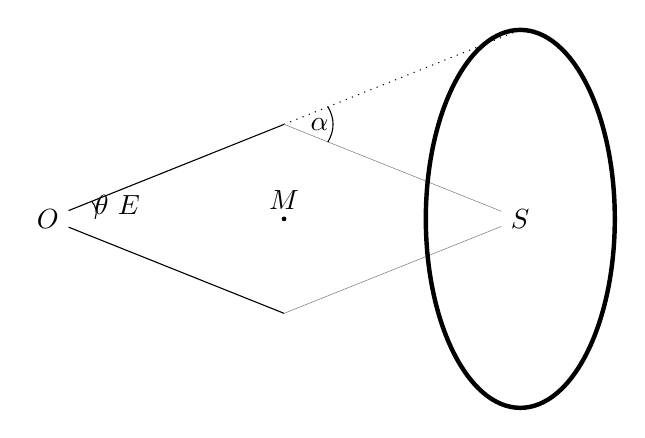
\begin{tikzpicture}[scale=0.6]
%\clip (0, -1) rectangle (10, 2.5);
    \node (O) at (0,0) {$O$}; 
    \coordinate (M) at (5,0);
\coordinate (P) at (5,2);
\coordinate (P') at (5,-2) {};
\node (S) at (10,0) {$S$};
\draw (O) to (P); \draw (O) to (P');
\coordinate (S') at (10,4);
\draw [dotted] (P) to (S');
\draw [bend right] (0:1) to (22:1);
\node at (11:1.5) {$\theta~E$};
\draw [help lines] (P) to (S) (P') to (S); 
\draw [bend left]($(P)+(22:1)$) to ($(P)+(-22:1)$);
\draw ($(P)+(0:.75)$) node {$\alpha$};
\draw [ultra thick] (S) ellipse (2 and 4);
\fill (M) circle (0.05) node [above] {$M$};

  \end{tikzpicture}
  \caption{The production of an \emph{Einstein ring}.}
  \label{fig:lensing-2}
\end{figure}

\section{Gravitational redshift}
\label{sec:grav-redsh-1}

Suppose light is emitted with the coordinates $(t_e,r_e)$ in the
Schwarzschild metric, and travels along a radial null geodesic to
reach an observer at an event $(t_o, r_o)$, then
\begin{equation}
  \label{eq:185}
  \dd{s}^2 = 0 = - \qty( 1 - \frac{2M}{r} ) \dd{t}^2 + \frac{\dd{r}^2}{1 - 2M/r}
\end{equation}
thus
\begin{equation}
  \label{eq:186}
  \int_{t_e}^{t_o} \dd{t} = t_o - t_e = \int_{r_e}^{r_o} \frac{\dd{r}}{1 - 2M/r}
\end{equation}
A wave with rest-frame frequency $\nu_0$ will have wavecrests leave
$r_e$ at $t_e$ and $t_e + \Delta t_e$, which reach $r_o$ at $t_o$ and
$t_o+\Delta t_e$, so the proper time difference between emissions is
\begin{equation}
  \label{eq:187}
  \Delta \tau_e = \Delta t_e \sqrt{1 - \frac{2M}{r_e}} \equiv \frac{1}{\nu_e} \equiv {\lambda_e}
\end{equation}
and between detections is
\begin{equation}
  \label{eq:188}
  \Delta \tau_o = \Delta t_e \sqrt{1 - \frac{2M}{r_o}} \equiv \frac{1}{\nu_o} \equiv \lambda_o
\end{equation}
so the redshift, $z$, is
\begin{equation}
  \label{eq:189}
  z = \frac{\lambda_o - \lambda_e}{\lambda_e} = \sqrt{ \frac{1-2M/r_o}{1-2M/r_e}} - 1 = \sqrt{\frac{r_e(r_o-R~S)}{r_o(r_e-R~S)}}-1
\end{equation}
for $R~S$ the Schwarzschild radius of the mass $M$.

\section{Gravitational time delay}
\label{sec:grav-time-delay}

Gravitational time delay has two constributions; a geometric one, and
a gravitational one, the Shapiro effect.

Taking the Schwarzschild invariant interval, and introducing 
\begin{equation}
  \label{eq:190}
  r = R \qty(1+\frac{M}{2R})^2
\end{equation}
then assuming a weak gravitational field, with $M \ll r$ and so $M \ll R$,
\begin{equation}
  \label{eq:191}
  r approx R \qty(1+ \frac{M}{R})
\end{equation}
and noting \[ 1 - \frac{2M}{r} = \frac{r-2M}{r} \]
we can produce the Schwarzschild metric in the form
\begin{equation}
  \label{eq:192}
\begin{split}
  \dd{s}^2 = - \qty( \frac{1-M/R}{1+M/R} ) \dd{t}^2 + \qty(\frac{1+M/R}{1-M/R}) \dd{r}^2 \\
+R^2 \qty( 1 + \frac{M}{R})^2 \qty[ \dd{\theta}^2 + \sin[2](\theta) \dd{\phi}^2]
\end{split}
\end{equation}
Using the binomial expansion,
\[ (1+x)^n \approx 1+ nx \]
and, noting that to first order $\dd{r} = \dd{R}$,
\begin{equation}
  \label{eq:194}
  \begin{split}
    \dd{s}^2 = - \qty(1 - \frac{2M}{R}) \dd{t}^2 \\
+ \qty(1+\frac{2M}{R}) \qty[ \dd{R}^2 + R^2 \dd{\theta}^2 + R^2 \sin[2](\theta) \dd{\phi}^2]
  \end{split}
\end{equation}
Then, defining the Cartesian coordinates,
\begin{equation}
  \label{eq:195}
  X = R \sin(\theta) \cos(\theta), \quad Y=R \sin(\theta) \sin(\phi), \quad Z = R \cos(\theta)
\end{equation}
and introducing the gravitational potential,
\[ \psi = - \frac{GM}{R} \]
The interval becomes
\begin{equation}
  \label{eq:196}
  \dd{s}^2 = -(1+2\psi) \dd{t}^2 + (1-2\psi) [\dd{X}^2 + \dd{Y}^2 + \dd{Z}^2]
\end{equation}

Consider a photon which propagates from a source at $A$ to an observer
at $B$ past a deflecting mass $M$, which is small, so we assume the
trajectory is straight in space, and align the coordinates so the
$z$-axis is along the line of propagation, so $\dd{x}=\dd{y}=0$, so
\begin{equation}
  \label{eq:197}
  \dd{s}^2 = - (1+2 \phi) \dd{t}^2 + (1-2 \psi) \dd{z}^2
\end{equation}
Since $\dd{s}^2 = 0$, to first order,
\begin{equation}
  \label{eq:198}
  \dd{t}^2 = \frac{1-2\psi}{1+2\psi} \dd{z}^2 \approx (1-2\psi)^2 \dd{z}^2
\end{equation}
Then $\int \dd{t} = \int(1-2\phi) \dd{z}$, so
\begin{equation}
  \label{eq:199}
  t~B - t~A = (z~B - z~A) - 2 \int_{z~A}^{z~B} \psi(z) \dd{z}
\end{equation}
With the second term being the time delay due to gravity,
\begin{equation}
  \label{eq:200}
  \delta t~{grav} = -2 \int_{z~A}^{z~B} \psi(z) \dd{z} \equiv -\frac{2}{c^3} \int_{z~A}^{z~B} \psi(z) \dd{z}
\end{equation}
%%% Local Variables: 
%%% mode: latex
%%% TeX-master: "../project"
%%% End: 


\chapter{Static Spherically Symmetric Stars}
\label{cha:einst-equat-stat}

In Newtonian theory the stability of stars is described in terms of
hydrostatic equilibrium. In the framework of General Relativity this
is similar, leading to the Oppenheimer-Volkoff equation.

\section{Components of the Einstein tensor}
\label{sec:comp-einst-tens}

The stellar interior will have a metric of the form
\[ \dd{s}^2 = -e^\nu \dd{t}^2 + e^{\lambda} \dd{r}^2 + r^2 \qty(
\dd{\theta}^2 + \sin[2](\theta) \dd{\phi}^2 )\] where $\nu$ and
$\lambda$ are functions of $r$. The Ricci tensor will have components
\begin{subequations}
\begin{equation}
  \label{eq:193}
  R_{tt} = \half e^{\nu-\lambda} \qty( \nu'' + \half \nu'^2 - \half \nu' \lambda' + \frac{2}{r} \nu')
\end{equation}
\begin{equation}
  \label{eq:201}
  R_{rr} = - \half \qty( \nu'' + \half \nu'^2 - \half \nu' \lambda' - \frac{2}{r} \lambda')
\end{equation}
\begin{equation}
  \label{eq:202}
  R_{\theta \theta} = 1 - e^{- \lambda} \qty( 1 + \frac{r}{2} ( \nu' - \lambda') )
\end{equation}
\begin{equation}
  \label{eq:203}
  R_{\phi \phi} = R_{\theta \theta} \sin[2](\theta)
\end{equation}
\end{subequations}
with all other components zero. The metric is orthogonal, so
\begin{subequations}
  \begin{align}
    g^{tt} &= - e^{- \nu} \\ g^{rr} &= e^{- \lambda} \\ g^{\theta \theta} &= r^{-2} \\ g^{\phi \phi} &= (r^2 \sin[2](\theta) )^{-1}
  \end{align}
\end{subequations} 
again, with all other terms zero.
The Ricci and metric tensors are orthogonal, so the Ricci scalar has the expression
\begin{equation}
  \label{eq:204}
  R = g^{\mu \nu} R_{\mu \nu} = g^{tt}R_{tt} + g^{rr} R_{rr} + g^{ \theta \theta} R_{\theta \theta} + g^{\phi \phi} R_{ \phi \phi}
\end{equation}
after making the appropriate substitutions, we find
\begin{equation}
  \label{eq:205}
  \begin{split}
    R = - e^{-\lambda} \qty[ \qty( \nu'' + \half \nu'^2 - \half \nu' \lambda' ) + \frac{\nu' - \lambda'}{r}]\\
{}+\frac{2}{r^2} \qty[1 - e^{- \lambda} \qty( 1+ \frac{(\nu' - \lambda')r}{2})]
  \end{split}
\end{equation}
The fully covariant Einstein tensor is
\[ G_{\mu \nu} = R_{\mu \nu} - \half g_{\mu \nu} R \]
so
\begin{subequations}
  \begin{align}
    G_{tt} &= \frac{e^{\nu}}{r^2} \qty[ 1+ e^{-\lambda} (r \lambda' -1) ] \\
G_{rr} &= \frac{\nu'}{r} - \frac{e^{\lambda}}{r^2} \qty( 1 - e^{- \lambda}) \\
G_{\theta \theta} &= r^2 e^{- \lambda} \qty[ \frac{\nu''}{2} + \frac{\nu'^2}{4} - \frac{\nu' \lambda'}{4} + \frac{\nu'-\lambda'}{2r}] \\
G_{\phi \phi} &= \sin[2](\theta) G_{\theta \theta}
  \end{align}
\end{subequations}

\section{Components of the energy-momentum tensor}
\label{sec:comp-energy-moment}

For a perfect fluid the energy-momentum tensor, in fully covariant
form has components
\[ T^{\mu \nu} = (\rho + P) u^{\mu} u^{\nu} + P g^{\mu \nu} \] for
$\rho$ the mass-energy density, and $P$ the pressure, while $u^{\mu}$
are the four velocity components of a fluid element. Seeking a static
solution has $u^{i} = 0, i = \set{1,2,3}$, so from the geodesic
equation
\begin{equation}
  \label{eq:206}
  g_{tt}(u^t)^2 = -1 \implies u^t = e^{- \frac{\nu}{2}}
\end{equation}
thus
\begin{subequations}
  \begin{align}
    T_{tt} &= \rho e^{\nu} \\
T_{rr} &= P e^{\lambda} \\
T_{\theta \theta} &= P r^2 \\
T_{\phi \phi} &= P r^2 \sin[2](\theta)
  \end{align}
\end{subequations}

\section{Einstein's equations}
\label{sec:einsteins-equations-1}

In fully covariant form
\[ G_{\mu \nu} = 8 \pi T_{\mu \nu} \]
so
\begin{subequations}
  \begin{align}
\label{eq:207}
    \frac{e^{\nu}}{r^2} \qty[  1+ e^{-\lambda} (r \lambda' -1) ] &= 8 \pi \rho e^{\nu} \\
\label{eq:208}
    \frac{\nu'}{r} - \frac{e^{\lambda}}{r^2} (1-e^-\lambda) &= 8 \pi P e^{\lambda} \\
\label{eq:209}
r^2 e^{-\lambda} \qty[ \frac{\nu''}{2} + \frac{\nu'^2}{4} - \frac{\nu' \lambda'}{4} + \frac{\nu'-\lambda'}{2r}] &= 8 \pi P r^2
  \end{align}
\end{subequations}

\section{Solution of the first Einstein equation}
\label{sec:solut-first-einst}

By cancelling the $e^{\nu}$ term in equation (\ref{eq:207}), and
rearranging,
\begin{equation}
  \label{eq:210}
  \dv{r} \qty[ r(1-e^{-\lambda})] = 8 \pi \rho r^2
\end{equation}
Then introducing the mass function, $m(r)$, defined as
\begin{equation}
  \label{eq:211}
  \dv{m}{r} = 4 \pi \rho r^2 = \half \dv{r} \qty[r (1-e^{-\lambda})]
\end{equation}
and integrating,
\begin{equation}
  \label{eq:212}
  r(1-e^{-\lambda}) = 2m +C 
\end{equation}
where $C$ is a constant of integration, equal to zero unless the star
is singular at $r=0$. Thus
\begin{equation}
  \label{eq:213}
  e^{-\lambda} = 1 - \frac{2m}{r}
\end{equation}

\section{The Oppenheimer-Volkoff equation}
\label{sec:oppenh-volk-equat}

Rearranging equation (\ref{eq:208}), with some straight-forward
algebra,
\begin{equation}
  \label{eq:214}
  \dv{\nu}{r} = e^{\lambda} \qty[8 \pi P r + \frac{1}{r} (1-e^{-\lambda})] = 2 \qty[\frac{4 \pi P r^3 + m}{r(r-2m)}]
\end{equation}
Then, considering conservation of mass-energy, $\tensor{T}{^{\alpha
    \beta}_{;\beta}} = \qty[(\rho +P) u^{\alpha}u^{\beta} + P
g^{\alpha \beta}]_{;\beta}= 0$, then
\begin{equation}
  \label{eq:215}
\begin{split}
  (\rho + P)_{;\beta} u^{\alpha} u^{\beta} + (\rho+P)(u^{\alpha})_{; \beta} u^{\beta} \\ + (\rho+P) u^{\alpha}(u^{\beta})_{; \beta} + P_{,\beta} g^{\alpha \beta} + Pg^{\alpha \beta}_{; \beta} = 0
\end{split}
\end{equation}
This is infact a set of four equations, as $\alpha$ is a free index,
so with just $\alpha \equiv r$,
\begin{equation}
  \label{eq:215}
\begin{split}
  (\rho + P)_{;\beta} u^{r} u^{\beta} + (\rho+P)(u^{r})_{; \beta} u^{\beta} \\ + (\rho+P) u^{r}(u^{\beta})_{; \beta} + P_{,\beta} g^{r \beta} + Pg^{r \beta}_{; \beta} = 0
\end{split}
\end{equation}
But since $u^r=0$ two of these terms vanish, and the derivatives of
the metric tensor are all zero, so the last term drops out too. We
then have the simplification
\begin{equation}
  \label{eq:216}
  ( \rho +P)(u^r)_{;t} u^t + \dv{P}{r} g^{rr} = 0
\end{equation}
then
\begin{equation}
  \label{eq:217}
  u^r_{;t} = \Gamma^r_{tt} u^t = \half \nu' e^{\nu-\lambda} e^{-\nu/2} = \half e^{-\lambda} \nu' e^{\nu/2}
\end{equation}
Thus
\begin{equation}
  \label{eq:218}
  \half(\rho + P) e^{-\lambda} \dv{\nu}{r} + e^{- \lambda} \dv{P}{r} = 0 \implies \dv{\nu}{r} = - \frac{2}{(\rho+P)} \dv{P}{r}
\end{equation}
and using this to eliminate $\nu'$ from equation (\ref{eq:214}),
\begin{equation}
  \label{eq:219}
  \dv{P}{r} = - \frac{(\rho + P)(4 \pi P r^3 + m)}{r(r-2m)}
\end{equation}
which is the \emph{Oppenheimer-Volkoff} equation. In the weak-field limit, $P \ll \rho$ implies $4 \pi P r^3 \ll m$, and the metric will be almost flat, so $m \ll r$, so this simplifies to
\begin{equation}
  \label{eq:220}
  \dv{P}{r} = - \frac{\rho m}{r^2}
\end{equation}
which is the Newtonian hydrostatic equilibrium equation.

\section{Solving the O-V equation}
\label{sec:solv-oppenh-volk}

There are three unknown functions in the O-V equation, $P(r)$,
$\rho(r)$, and $m(r)$, but the latter two are related, so we need an
additional relation, an equation of state, to link all three, in the form
\[ P(r) = P(\rho(r)) \]
For a fluid which is in local thermodynamic equilibrium there is always a relation between pressure, density, and entropy, of the form
\[ P=P(\rho,S) \] In most astrophysical situations we can regard $S$
as constant. In practice, to solve this system we need boundary
conditions.

Take $P=P_0$ and $m=0$ at $r=0$, and integrate outwards to $P=0$ at
the surface of the star, where $r=R$ and $m=M$, where $M$ is the mass
constant in the exterior Schwarzschild metric. This then allows us to
find $\nu$ and $\lambda$ to form a complete expression for the metric
inside the star. The effect of GR compared to Newtonian mechanics will
be to steepen the pressure gradient within the star.

\section[Constant density star solution]{An exact solution for a star with constant density}
\label{sec:an-exact-solution}

Suppose that the density is constant, and $\rho=\rho_0$ (implying,
rather concerningly, an infinite sound speed!), and integrating
equation (\ref{eq:211}), and retrieve
\begin{equation}
  \label{eq:221}
  m(r) = \frac{4}{3} \pi \rho_0 r^3
\end{equation}
This can be substituted into the O-V equation, giving
\begin{equation}
  \label{eq:222}
  \dv{P}{r} = - \frac{4}{3} \pi r \frac{(\rho_0+P)(\rho_0 + 3 P)}{(1 - \frac{8 \pi \rho_0 r^2}{3})}
\end{equation}
thus
\begin{align*}
  \label{eq:223}
  \frac{\dd{P}}{(\rho_0 +P)(\rho_0 + 3P)} &= \frac{1}{2 \rho_0} \qty[\frac{3 \dd{P}}{(\rho_0 + 3P)} - \frac{\dd{P}}{(\rho_0 +P)}] \\ &= - \frac{4 \pi}{3} \frac{r \dd{r}}{\qty(1 - \frac{8 \pi \rho_0 r^2}{3})}
\end{align*}
and integrating both sides,
\begin{equation}
  \label{eq:224}
  \log( \rho_0 + 3P) - \log(\rho_0 + P) = \half \log(1 - \frac{8 \pi \rho_0 r^2}{3}) + C
\end{equation}
for a constant $C$, which can be written
\begin{equation}
  \label{eq:225}
  \frac{\rho_0 + 3P}{\rho_0+P} = A \qty( 1 - \frac{8 \pi \rho_0 r^2}{3})^{1/2}
\end{equation}
when $r=0$ we have $P=P_0$, so we can express $A$ in terms of density and central pressure,
\[ A = \frac{\rho_0 + 3 P_0}{\rho_0 +P_0} \]
Then
\begin{align}
  \label{eq:226}
  \frac{\rho_0 + 3P}{\rho_0 + P} &= \frac{\rho_0 + 3P_0}{\rho_0 + P_0}  \qty( 1 - \frac{8 \pi \rho_0 r^2}{3})^{1/2} \nonumber\\
&=  \frac{\rho_0 + 3P_0}{\rho_0 + P_0} \qty( 1 - \frac{2m}{r})^{1/2}
\end{align} at the surface of the star $P=0$ so the left hand reduces
to $1$, so
\begin{equation}
  \label{eq:227}
  \frac{\rho_0 + 3P_0}{\rho_0 + P_0} \qty( 1 - \frac{2m}{r})^{1/2} = 1
\end{equation}
for $M$ the Schwarzschild mass, and $R$ is the coordinate radius of
the star. We can obtain an expression for $P$ as a function of $r$ by rearranging,
\begin{equation}
  \label{eq:228}
  P_0 = \frac{\rho_0 \qty[ 1 - \qty( 1 - \frac{2M}{R} )^{1/2}]}{3 \qty( 1 - \frac{2M}{R})^{1/2} - 1}
\end{equation}

\section{Buchdahl's Theorem}
\label{sec:buchdahls-theorem}

From equation (\ref{eq:228}), it can be seen that as $P_0 \to \infty$
when $3 \qty(1- \frac{2M}{R})^{1/2} \to 1$, that is, when $M/R \to
4/9$. Clearly there can be no static star with uniform density with a
radius smaller than $9M/4$, as they would require an infinite internal
pressure. If we require the exterior metric to be well-behaved then
stars with a radius less than $2M$ should be excluded, as the
Schwarzschild metric misbehaves at this point, with timelike intervals
becoming spacelike, and vice versa.

As a result we can exclude the possibility of a uniform static star
with these properties, and \emph{Buchdahl's theorem} is a rigorous
proof of this.



%%% Local Variables: 
%%% mode: latex
%%% TeX-master: "../project"
%%% End: 


\chapter{Gravitational Radiation}
\label{cha:grav-radi}

\section{Non-stationarity}
\label{sec:non-stationarity}

A non-stationary metric has a metric with some dependence on the time
coordinate, $t$, and an important consequence of these metrics is that
they permit gravitational radiation.

\section{Weak fields}
\label{sec:weak-fields}

In the absence of energy and matter spacetime is flat and
Mikowskian. We can introduce a perturbation, however, to make the
metric ``nearly-flat'', with the form
\begin{equation}
  \label{eq:229}
  g_{\alpha \beta} = \eta_{\alpha \beta} + h_{\alpha \beta}
\end{equation}
Where $\eta_{\alpha \beta} = \diag(-1,1,1,1)$ is the Minkowski metric,
and $\abs{h_{\alpha \beta}} \ll 1$. This spacetime still obeys Lorentz
transformations, $\Lambda$, so
\begin{equation}
  \label{eq:1}
  g'_{\alpha \beta} = \Lambda_{\alpha'}^{\mu} \Lambda_{\beta'}^{\nu} g_{\mu \nu} =  \Lambda_{\alpha'}^{\mu} \Lambda_{\beta'}^{\nu} \eta_{\mu \nu} +  \Lambda_{\alpha'}^{\mu} \Lambda_{\beta'}^{\nu} h_{\mu \nu} = \eta_{\alpha \beta}' + h_{\alpha \beta}'
\end{equation} 
Gauge transformations can also be applied, with the form
\begin{equation}
  \label{eq:2}
  x'^{\alpha} = x^{\alpha} + \xi^{\alpha}(x^{\beta})
\end{equation}
for $\xi^{\alpha}$ functions of the coordinates $\set{x^{\alpha}}$, and so
\begin{equation}
  \label{eq:3}
  \Lambda_{\alpha}^{\beta} = \delta^{\alpha}_{\beta} + \xi_{,\beta}^{\alpha}
\end{equation}
We can demand that the $\xi^{\alpha}$ are small, so
\[ \abs{\xi^{\alpha}_{,\beta}} \ll 1 \quad \forall \alpha,\beta\]
Thus by the chain rule
\begin{equation}
  \label{eq:5}
  \Lambda_{\alpha}^{\gamma} = \delta^{\alpha}_{\gamma} - \Lambda^{\gamma}_{\beta} \Lambda^{\beta}_{\alpha} \approx \delta^{\alpha}_{\gamma} - \xi_{,\gamma}^{\alpha} 
\end{equation}

If the unprimed coordinate system is nearly Lorentz, then
\begin{align*}
  g'_{\alpha \beta} &= \Lambda_{\alpha}^{\nu} \Lambda_{\beta}^{\nu} g_{\mu \nu} \\
&= \qty( \delta_{\alpha}^{\mu} \delta_{\beta}^{\nu} - \xi_{,\alpha}^{\mu} \delta_{\beta}^{\nu} - \xi^{\nu}_{,\beta} \delta_{\alpha}^{\mu} ) \eta_{\mu \nu} + \delta_{\alpha}^{\mu} \delta_{\beta}^{\nu} h_{\mu \nu} \\
&= \nu_{\alpha \beta} + h_{\alpha \beta} -\xi_{\alpha, \beta} - \xi_{\beta , \alpha}
\end{align*}
This has the same form as equation (\ref{eq:229}) provided that
\[ h'_{\alpha \beta} = h_{\alpha \beta} - \xi_{\alpha, \beta} - \xi_{\beta, \alpha} \]

Clearly the new primed system is also nearly Lorentz.

\section{Einstein's equations in weak fields}
\label{sec:einst-equat-weak}

In the nearly Lorentz system we have a restricted number of coordinate
transforms which can be used so that the resulting system is still
nearly Lorentz.

To the first order for small perturbations the Riemann-Christoffel
tensor for a nearly-flat space is 
\begin{equation}
  \label{eq:7}
  \tensor{R}{_{\alpha \beta \gamma \delta}} = \half \qty( h_{\alpha \delta, \beta \gamma}+ h_{\beta \gamma, \alpha \delta} - h_{\alpha \gamma, \beta \delta} - h_{\beta \delta,\alpha \gamma} )
\end{equation}
The Ricci tensor can then be obtained,
\begin{equation}
  \label{eq:8}
  R_{\mu \nu} = \half \qty( h^{\alpha}_{\mu, \nu \alpha} + h^{\alpha}_{\nu, \mu \alpha} - h_{\mu \nu,\alpha}^{,\alpha} - h_{, \mu \nu} )
\end{equation} for $h \equiv h^{\alpha}_{\alpha} = \eta^{\alpha \beta} h_{\alpha \beta}$. Also the Ricci scalar,
\begin{equation}
  \label{eq:9}
  R = \eta^{\alpha \beta} R_{\alpha \beta}
\end{equation}
allowing the Einstein tensor to be found,
\begin{align}
  G_{\mu \nu} &= R_{\mu \nu} - \half \eta_{\mu \nu} R \nonumber\\
&= \half \qty[h_{\mu \alpha,\nu}^{,\alpha} + h_{\nu \alpha,\mu}^{, \alpha} - h_{\mu \nu,\alpha}^{,\alpha} - h_{, \mu \nu} - \eta_{\mu \nu} \qty( h_{\alpha \beta}^{,\alpha \beta} - h_{,\beta}^{,\beta})]
\end{align}
By rescaling the metric perturbations,
\begin{equation}
  \label{eq:10}
  \bar{h}_{\mu \nu} \equiv h_{\mu \nu} - \half \eta_{\mu \nu} h
\end{equation}
then 
\begin{equation}
  \label{eq:11}
  G_{\mu \nu} = - \half \qty[ \bar{h}_{\mu \nu, \alpha}^{,\alpha} + \eta_{\mu \nu}\bar{h}_{\alpha \beta}^{, \alpha \beta} - \bar{h}_{\mu \alpha, \nu}^{,\alpha} - \bar{h}_{\nu \alpha, \mu}^{, \alpha}]
\end{equation}
Since
\[ G_{\mu \nu} = 8 \pi T_{\mu \nu} \] it follows
\begin{equation}
  \label{eq:12}
  - \bar{h}_{\mu \nu,\alpha}^{,\alpha} - \eta_{\mu \nu}^{,\alpha \beta} + \bar{h}_{\mu \alpha, \nu}^{, \alpha} + \bar{h}_{\nu \alpha, \mu}^{,\alpha} = 16 \pi T_{\mu \nu}
\end{equation}
We can always find a gauge in which the last three terms are
zero---the Lorentz gauge, which is equivalent to adopting the
coordinate system in which \[ \bar{h}^{\mu \alpha}_{, \alpha} = 0 \]
(i.e. the metric with the divergence of perturbations equal to zero), thus
\begin{equation}
  \label{eq:13}
  - \bar{h}_{\mu \nu, \alpha}^{,\alpha} = 16 \pi T_{\mu \nu}
\end{equation}

\subsection{Solutions in free space}
\label{sec:solutions-free-space}

Solutions in free space will be solutions of 
\begin{equation}
  \label{eq:14}
   \eta^{\alpha \alpha } \bar{h}_{\mu \nu, \alpha \alpha} = \bar{h}_{\mu \nu, \alpha}^{,\alpha} = 0
\end{equation}
which written in slightly more familiar notation is
\begin{equation}
  \label{eq:15}
  \qty( - \pdv[2]{t} + \nabla^2 ) \bar{h}_{\mu \nu} = 0
\end{equation}
moving out of geometrised units, setting $\eta^{00} = -c^{-2}$, then
\begin{equation}
  \label{eq:16}
   \qty( - \pdv[2]{t} + c^2\nabla^2 ) \bar{h}_{\mu \nu} = 0
\end{equation}
This has the form of a wave equation.

\section{Plane wave solutions}
\label{sec:plane-wave-solutions}

\section{Free particles}
\label{sec:free-particles}

\section{Gravitational wave amplitude}
\label{sec:grav-wave-ampl}

\section{Quadrupolarity}
\label{sec:quadrupolarity}



%%% Local Variables: 
%%% mode: latex
%%% TeX-master: "../project"
%%% End: 



\chapter{Black Holes}
\label{cha:black-holes}

\chapter{Cosmology}
\label{cha:cosmology}



\appendices


\end{document}



%%% Local Variables: 
%%% mode: latex
%%% TeX-master: t
%%% End: 
